\documentclass[12pt, a4paper]{article}

% ----- PACKAGES -----
\usepackage[T1]{fontenc} % Added for proper font metric handling
\usepackage[utf8]{inputenc}
\usepackage{geometry}
\usepackage{float}
\geometry{a4paper, margin=1in}
\usepackage{mathptmx} % Sets font to Times New Roman
\usepackage{graphicx}
\usepackage{titlesec}
\usepackage[round]{natbib}
\usepackage{setspace}
\usepackage{amsmath}
\usepackage{amssymb}
\usepackage{booktabs}
\usepackage{indentfirst}
\usepackage[hypertexnames=false]{hyperref}
\hypersetup{hidelinks}
\usepackage{enumitem}


\setlength{\parindent}{1.25cm}
\setlength{\parskip}{0.5em}
% Adjust heading formatting to match standard report styles
\titleformat{\section}{\normalfont\Large\bfseries}{\thesection}{1em}{}
\titleformat{\subsection}{\normalfont\large\bfseries}{\thesubsection}{1em}{}
\setcounter{MaxMatrixCols}{20}
\begin{document}
	
	% ==========================================
	% FRONT MATTER
	% ==========================================
	\pagenumbering{roman}
	
	% --- TITLE PAGE ---
	\begin{titlepage}
		\centering
		
		
		% Project Title (Size 18, Times New Roman, Bold)
		\vspace*{1cm}
		{\fontsize{18}{22}\selectfont\textbf{Design and Validation of a Scalable Decentralised Control Architecture for Multi Zone HVAC Systems}\par}
		
		\vspace{1.5cm}
		
		% Module Name (Size 14, Times New Roman, Bold)
		{\fontsize{14}{17}\selectfont\textbf{ME420: Mechanical Engineering Individual Research Project}\par}
		
		\vspace{1.5cm}
		
		% Submitted by (Size 14, Times New Roman, Bold)
		{\fontsize{14}{17}\selectfont\textbf{Submitted by}\par}
		\vspace{0.5cm}
		% Names, Reg. Nos., Group No. (Size 14, Times New Roman)
		{\fontsize{14}{17}\selectfont
			W.S.P.Y.J.C. Yapa (Reg. No: E/20/452)\par}
		
		\vspace{1.5cm}
		
		% "in" (Size 14, Times New Roman, Bold)
		{\fontsize{14}{17}\selectfont\textbf{in}\par}
		\vspace{0.5cm}
		% Partial fulfillment... (Size 14, Times New Roman)
		{\fontsize{14}{17}\selectfont
			partial fulfillment of the requirements for the degree\\
			Bachelor of the Science of Engineering\par}
		
		\vspace{1.5cm}
		
		% University Logo
		
\includegraphics[width=4cm]{images/university_logo.png} % Uncomment and upload logo
		
		\vspace{1.5cm}
		
		% Department Details (Size 14, Times New Roman, Bold)
		{\fontsize{14}{17}\selectfont\textbf{Department of Mechanical Engineering\\
				Faculty of Engineering, University of Peradeniya}\par}
		
		\vfill
		
		% Date (Size 14, Times New Roman)
		{\fontsize{14}{17}\selectfont
			August 16, 2026\par}
		
		
		
	\end{titlepage}
	% --- EXECUTIVE SUMMARY ---
	\section*{Executive Summary}
	\addcontentsline{toc}{section}{Executive Summary}
	Conventional HVAC control systems are primarily designed around dry-bulb temperature regulation, typically using PID based strategies. Although it is effective for single variable temperature tracking, such approaches do not explicitly coordinate temperature, humidity, and CO$_2$ concentration, which are the three principal variables governing indoor comfort and air quality. This limitation is particularly challenging in VAV systems, where all three variables are influenced through a common airflow actuator while each state is influenced by different dynamics and respond to different disturbance sources. Consequently, maintaining acceptable IAQ requires a coordinated multivariable control strategy rather than independent temperature regulation.
	
	The challenge becomes more significant in multi-zone buildings. A centralised MPC can formulate the complete multivariable IAQ problem, but its computational burden increases with the number of zones. In addition, a centralised approach requires a detailed model representing the complete building, making its formulation and tuning increasingly difficult when the number of zones, layout, or building characteristics change. These limitations motivate a control architecture that can distribute the computational effort while retaining coordination over shared AHU resources.
	
	This project develops, implements, and validates a scalable decentralised control architecture for multi-zone HVAC systems that jointly maintains temperature, humidity, and CO$_2$ within prescribed comfort and IAQ regions. Each zone employs an augmented Extended Kalman Filter with a grey-box model to estimate hidden states, disturbances, occupancy, and model parameters online. A two phase sequential MPC determines the required VAV airflow and generates an optimal supply-air request. A supervisory AHU Coordinator then arbitrates the requests from all zones through a quadratic programme governing the supply air condition for the whole building.
	
	Validation is conducted using a five-zone EnergyPlus simulation and a physical single zone experimental test bench. Results demonstrate effective maintenance of the three IAQ variables under varying disturbances while distributing computational effort across zones. The primary contribution is therefore a scalable framework that is easy to implement in practice for multivariable IAQ control in a multi-zone HVAC system.
	\newpage
	
	% --- ACKNOWLEDGMENTS ---
	\section*{Acknowledgments}
	\addcontentsline{toc}{section}{Acknowledgments}
	
	First and foremost, I would like to express my deepest gratitude to my project supervisor, Dr. D. H. S. Maithripala, for his invaluable guidance, continuous encouragement, and unwavering support throughout this project. His technical insight, constructive criticism, and willingness to discuss and clarify challenging aspects of the work were instrumental in its successful completion.
	
	I would also like to express my sincere appreciation to the Head of the Department and all the professors and lecturers of the Department of Mechanical Engineering, University of Peradeniya, for providing the knowledge, academic guidance, and valuable feedback that contributed to the development of this project. Their continued support have been invaluable throughout my undergraduate studies. 
	
	My sincere thanks are extended to the technical staff of the Department of Mechanical Engineering,  for their assistance and support during the practical and experimental aspects of the project. Their technical guidance and facilitation of the necessary resources greatly contributed to the successful implementation of the work.
	
	Finally,  I am also grateful to my colleagues and friends for their valuable discussions, suggestions, encouragement, and support throughout the project. Their different perspectives and feedback helped me identify problems and improve the quality of the work.
	

	
	\newpage
	
	% --- DECLARATION ---
	\newpage
	\section*{Declaration}
	\addcontentsline{toc}{section}{Declaration}
	
	I declare that this report does not incorporate, without acknowledgement, any material previously submitted for any other Degree or Diploma. To the best of my knowledge and belief, it does not contain any material previously published or written by another person or myself except where due references are made. It has not been accepted for any other course and is not being concurrently submitted to any other person.
	
	\vspace{2.5cm}
	
	\noindent
	\begin{minipage}[t]{0.6\textwidth}
		Signature of candidate \\[1.5cm]
		....................................................... \\[0.5cm]
		Name of candidate \\[0.5cm]
		W.S.P.Y.J.C. Yapa
	\end{minipage}%
	\begin{minipage}[t]{0.4\textwidth}
		Date: August 16, 2026
	\end{minipage}
	
	\vspace{3cm}
	
	\noindent Countersigned by:
	
	\vspace{1cm}
	
	\noindent
	\begin{minipage}[t]{0.6\textwidth}
		Signature of supervisor \\[1.5cm]
		....................................................... \\[0.5cm]
		Name of Supervisor \\[0.5cm]
		Dr. D. H. S. Maithripala
	\end{minipage}%
	\begin{minipage}[t]{0.4\textwidth}
		Date: ......./......./.......
	\end{minipage}
	\newpage


	\newpage
	
	% --- TABLE OF CONTENTS & LISTS ---
	\tableofcontents
	\newpage
	\listoffigures
	\addcontentsline{toc}{section}{List of Figures}
	\newpage
	\listoftables
	\addcontentsline{toc}{section}{List of Tables}
	\newpage
	
	% --- ABBREVIATIONS ---
	\section*{Abbreviations}
	\addcontentsline{toc}{section}{Abbreviations}
	
	% labelwidth controls the gap size. Adjust "2.5cm" if needed.
	\begin{description}[align=left, labelwidth=2.5cm, leftmargin=!]
		\item[ADAL] Accelerated Distributed Augmented Lagrangian
		\item[AHU] Air Handling Unit
		\item[ANN] Artificial Neural Network
		\item[ASHRAE] American Society of Heating, Refrigerating and Air-Conditioning Engineers
		\item[CO$_2$] Carbon Dioxide
		\item[DAQ] Data Acquisition
		\item[DX] Direct Expansion
		\item[EKF] Extended Kalman Filter
		\item[eCO$_2$] Equivalent Carbon Dioxide
		\item[ESP-IDF] Espressif IoT Development Framework
		\item[HVAC] Heating, Ventilation, and Air Conditioning
		\item[IAQ] Indoor Air Quality
		\item[I2C] Inter-Integrated Circuit
		\item[IDF] Input Data File
		\item[MPC] Model Predictive Control
		\item[OA] Outdoor Air
		\item[OSQP] Operator Splitting Quadratic Program Solver
		\item[PCB] Printed Circuit Board
		\item[PID] Proportional-Integral-Derivative
		\item[PI] Proportional-Integral
		\item[PWM] Pulse Width Modulation
		\item[QP] Quadratic Programme
		\item[RC] Resistance-Capacitance
		\item[RH] Relative Humidity
		\item[SAT] Supply Air Temperature
		\item[VAV] Variable Air Volume
	\end{description}


	\newpage
	
	\pagenumbering{arabic}
	
	\section{Introduction}
	
	Heating, ventilation, and air conditioning (HVAC) systems play a central role in maintaining acceptable indoor environmental conditions. In conventional buildings, however, HVAC control is primarily based on temperature regulation, with thermostats and PID controllers designed to track a prescribed dry-bulb temperature set-point \citep{harroldAutomaticControlsBuilding1988}. While this approach is effective for basic temperature regulation, it does not explicitly address other important indoor air quality (IAQ) variables, particularly humidity and CO$_2$ concentration. Maintaining acceptable indoor conditions therefore requires consideration of multiple interacting variables rather than temperature control alone.
	
	The simultaneous regulation of temperature, humidity, and CO$_2$ presents a fundamental control challenge in VAV systems. These variables are coupled through the thermal, moisture, and contaminant dynamics of the zone, yet their regulation is influenced by a common airflow actuator. Furthermore, they respond on different time scales and are affected by disturbances such as occupancy, internal heat and moisture generation, and outdoor conditions. A controller that independently regulates individual variables may therefore fail to maintain the overall IAQ condition, particularly when actuator limitations and interactions between the controlled variables are considered.
	
	Model-predictive control (MPC) provides a systematic framework for addressing these interactions by predicting future system behaviour and explicitly incorporating comfort and physical constraints into the control problem \citep{camachoModelPredictiveControl2007, aframTheoryApplicationsHVAC2014}. However, applying a fully centralised MPC to a multi-zone building introduces a different challenge. As the number of zones increases, the optimisation problem becomes larger and computationally more demanding \citep{yangHVACEnergyCost2019}. The centralised formulation also requires a model representing the complete building, making the controller increasingly difficult to formulate, tune, and adapt when the number of zones or building characteristics change.
	
	This project therefore develops, implements, and validates a scalable decentralised control architecture for multi-zone HVAC systems. The proposed approach distributes state estimation and zone-level control across individual rooms while retaining supervisory coordination of the shared air-handling unit. Each zone jointly considers temperature, humidity, and CO$_2$ within prescribed comfort and IAQ limits, while the supervisory layer coordinates the competing requirements of multiple zones. The objective is to demonstrate that multivariable IAQ control can be achieved without relying on a single increasingly complex centralised controller, providing a more practical framework for extending advanced HVAC control to multi-zone buildings.
	
	\newpage
	\subsection{Aims and Objectives}
	
	The primary aim of this project is to design, implement, and validate a scalable, decentralised control architecture for multi-zone HVAC systems that jointly maintains indoor temperature, humidity, and CO$_2$ within comfort bounds while minimising mechanical actuation effort. This aim is pursued through the following specific objectives.
	
	\begin{itemize}
		\item Develop a dynamic grey-box thermal and mass-balance model for a single zone that is suitable for real-time predictive control.
		\item Design an augmented Extended Kalman Filter that simultaneously estimates unmeasured physical states, lumped environmental disturbances, and unknown building parameters online.
		\item Implement an actuation minimising dead-band MPC that optimises VAV airflow and formulates an optimal supply air request for the central layer.
		\item Design a supervisory AHU Coordinator that arbitrates supply requests from all zones into a single solution.
		\item Validate the full multi-zone architecture in a five-zone EnergyPlus simulation under realistic occupancy and weather conditions.
		\item Verify zone-level controller behaviour on a physical single-zone experimental test-bench, confirming practical deployability beyond simulation.
	\end{itemize}
	
	\subsection{Scope}
	The scope of this project include the full design and validation pipeline of the two-layer control architecture. At the zone level, this includes the development of the thermal model, the augmented EKF state estimator, the two-phase sequential MPC, and the ideal supply air request formulation. At the supervisory level, it includes the multi-zone arbitration implemented in the AHU Coordinator. On the validation side, the scope covers both the EnergyPlus five-zone simulation and the physical single-zone test-bench, including the associated sensing hardware, embedded firmware, and real-time monitoring interface.
	
	The scope does not extend to multi-AHU configurations, fault detection and diagnosis, or the data-driven system identification pipeline required to automatically extract RC model parameters from raw building sensor logs. These are identified as natural extensions of the current work but fall outside the boundary of this project.
	
	\subsection{Intended Beneficiaries}
	
	The architecture developed in this project is primarily intended to benefit HVAC design engineers by providing a modular and scalable control framework that reduces the need to develop and redesign a complete control strategy for each individual building. Building owners and facility operators can benefit from a more practical pathway for deploying advanced multi-zone HVAC control without the complexity of developing a fully centralised controller for thier building. Ultimately, building occupants are the direct beneficiaries through improved and more consistent indoor air quality, with temperature, humidity, and CO$_2$ jointly maintained within prescribed operating regions. The work also provides a validated reference architecture for researchers working on decentralised building control, state estimation, and scalable multi-zone optimisation, supporting further development of practical IAQ control strategies.


	\subsection{Approach}
	
	The approach taken is hierarchical and modular. Each zone operates an autonomous local controller that builds a predictive model of its own thermal and air quality dynamics, estimates hidden quantities it cannot directly measured, and computes the minimum airflow needed to keep conditions within comfort bounds. That local controller also formulates an informed request to the central air handling unit, describing the supply air conditions that would best serve its needs. A supervisory coordinator then arbitrates across all zones simultaneously, finding the single set of physical coil and damper commands that best serves the building as a whole.
	
	Validation is carried out through two complementary streams. A five-zone EnergyPlus simulation that tests the full multi-zone architecture under varied occupancy schedules and weather conditions, and a physical single-zone experimental test-bench that confirms the algorithms translate faithfully from code to hardware. Together these two streams address the deployment gap that afflicts much of the academic literature on building control, where promising methods are validated only in simulation and never tested on real equipment.
	
	\subsection{Assumptions}
	
	A foundational assumption underpinning the entire approach is that the complex and largely unmeasurable disturbances acting on a building solar heat gain, infiltration, inter-zone air exchange can be captured sufficiently well by real-time disturbance estimation rather than explicit physical modelling. The EKF disturbance observer is designed to absorb these effects as slowly-varying lumped inputs, which is valid provided disturbances evolve on timescales longer than the observer's convergence time. A secondary assumption is that the linearisation of zone dynamics around the current EKF operating point, performed at each time step, introduces negligible error relative to the disturbance estimation uncertainty. 
	
	\subsection{Expected Outcomes}
	
	\noindent The successful execution of this project is expected to achieve the following outcomes.
	
	\begin{itemize}
		\item \textbf{A scalable control framework : } in which adding or removing thermal zones requires no redesign of any other part of the system.
		\item \textbf{Joint IAQ regulation :} demonstrating that temperature, humidity, and CO$_2$ can be maintained simultaneously within ASHRAE defined comfort bounds using a single VAV actuator per zone.
		\item \textbf{Practical hardware deployment :} bridging the gap between simulation and reality through a functional embedded controller network with real-time telemetry.
	\end{itemize}
	
	\newpage

	\section{Background}
	
	
	\subsection{Conventional HVAC Control Strategies and their Limitations}
	
	Although advanced control methods can theoretically provide coordinated and optimal regulation of complex HVAC systems, practical building control remains dominated by relatively simple feedback strategies, particularly PI and PID controllers. Their simplicity, robustness, and ease of implementation make them attractive for real world deployment, but they are primarily suited to regulating individual variables and do not naturally account for the coupled behaviour of temperature, humidity, and CO$_2$. This subsection reviews the main control approaches used in HVAC systems and examines the practical limitations that motivate the need for a scalable multivariable control architecture.
	
	\subsubsection{Classical Control}
	
	Conventional HVAC regulation relies on on-off switching, proportional-integral-derivative (PID) loops, and time scheduling strategies \citep{harroldAutomaticControlsBuilding1988}. These methods are simple, robust, and inexpensive to implement, which explains their continued dominance in practice \citep{naiduAdvancedControlStrategies2011}. However, as Table~\ref{tab:classical_limits} summarises, they face fundamental structural limitations when applied to modern multi-zone buildings \citep{balaliEnergyModellingControl2023}.
	
	\begin{table}[h]
		\centering
		\caption{Limitations of Classical HVAC Control}
		\label{tab:classical_limits}
		\begin{tabular}{lp{8cm}}
			\toprule
			\textbf{Limitation} & \textbf{Consequence} \\
			\midrule
			Single-variable regulation & Temperature is controlled, but humidity and CO$_2$ ignored \\
			No predictive capability & Reacts to disturbances after they occur \\
			No constraint handling & Cannot enforce actuator limits or comfort bounds explicitly \\
			Poor multi-variable coupling & Cannot manage interacting temperature, humidity, and CO$_2$ \\
			Fixed scheduling & No adaptation to real-time occupancy or weather \\
			\bottomrule
		\end{tabular}
	\end{table}
	
	The most critical limitation for this project is that classical controllers almost universally regulate dry-bulb temperature only, leaving relative humidity and indoor CO$_2$ concentration entirely unmanaged. As described in Section~\ref{sec:iaq}, true indoor air quality requires all three to be maintained simultaneously.
	
	\subsubsection{Intelligent and Soft Computing Approaches}
	
	Fuzzy logic controllers, artificial neural networks (ANN), and genetic algorithms have been investigated as alternatives to address the non-linearities and adaptability shortcomings of classical PID control \citep{singhFuzzyModelingControl2009, kalogirouArtificialNeuralNetworks2009, dounisAdvancedControlSystems2009}. These methods improve local component performance and can approximate non-linear system behaviour without requiring an explicit physical model \citep{naiduAdvancedControlStrategies2011}. However, they share a set of structural deficiencies that make them unsuitable as the primary control framework for this project.
	
	\begin{itemize}
		\item \textbf{No explicit physical constraint handling} - Comfort bounds and actuator limits cannot be formally enforced.
		\item\textbf{ No predictive optimisation over a future horizon }- The controller reacts rather than anticipates.
		\item \textbf{Poor scalability} - Performance degrades as system complexity grows.
		\item \textbf{Uninterpretable decisions} - The control action cannot be explained in physical terms, complicating commissioning and fault diagnosis.
	\end{itemize}
	
	\subsubsection{Model Predictive Control}
	
	Model Predictive Control (MPC) has emerged as the most theoretically rigorous advanced control framework for HVAC applications \citep{aframTheoryApplicationsHVAC2014, wangSupervisoryOptimalControl2008}. At each time step, MPC solves an optimisation problem over a receding prediction horizon, selecting the sequence of control actions that minimises a cost function while satisfying explicit constraints on states and inputs \citep{camachoModelPredictiveControl2007, qinSurveyIndustrialModel2003}. Table~\ref{tab:mpc_advantages} summarises the key properties that make MPC particularly well suited to HVAC.
	
	\begin{table}[h]
		\centering
		\caption{Advantages of MPC for HVAC Control}
		\label{tab:mpc_advantages}
		\begin{tabular}{lp{8cm}}
			\toprule
			\textbf{Property} & \textbf{Relevance to HVAC} \\
			\midrule
			Anticipatory control & Responds to predicted occupancy and weather rather than reacting after the fact \\
			Explicit constraint enforcement & Comfort bounds, actuator limits, and slew rates are hard constraints in the optimisation \\
			Multi-objective optimisation & Energy minimisation and comfort maintenance are jointly optimised \\
			Disturbance forecasting & Known disturbances (e.g., scheduled occupancy) are incorporated into predictions \\
			Multi-variable capability & Temperature, humidity, and CO$_2$ can be managed within a single formulation \\
			\bottomrule
		\end{tabular}
	\end{table}
	
	Despite these advantages, centralised MPC faces a fundamental scalability barrier in multi-zone buildings. As the number of zones grows, inter-zone thermal coupling and shared AHU constraints create a non separable optimisation problem which also cause to dimensionality grow \citep{yangHVACEnergyCost2019}. Current literature states that this computational bottleneck is the primary reason comprehensive MPC deployments in large commercial buildings remain rare \citep{aframTheoryApplicationsHVAC2014, balaliEnergyModellingControl2023}.
	
	\subsection{The Coupled Nature of Indoor Air Quality Regulation}
	\label{sec:iaq}
	
	A critical deficiency in current methods is their treatment of indoor environmental quality as a single-variable temperature problem. In reality, occupant health, comfort, and cognitive performance depend on three coupled quantities that must be maintained simultaneously \citep{aframTheoryApplicationsHVAC2014}, as defined in Table~\ref{tab:iaq_bounds}.
	
	The challenge is that all three variables in a VAV-served zone are driven through a single actuator the VAV damper. Temperature, humidity, and CO$_2$ each respond on different timescales, are driven by different disturbance sources (occupant heat gain, moisture generation, and respiration respectively), and have partially conflicting control requirements \citep{wangSupervisoryOptimalControl2008}. This makes their joint regulation a fundamentally \textit{underactuated} problem. There are three output constraints and one control input per zone. No classical or soft-computing approach in the literature formulates this problem explicitly \citep{naiduAdvancedControlStrategies2011, dounisAdvancedControlSystems2009}.
	
	\begin{table}[h]
		\centering
		\caption{Indoor Environmental Quality Comfort Bounds}
		\label{tab:iaq_bounds}
		\begin{tabular}{llll}
			\toprule
			\textbf{Variable} & \textbf{Target Range} & \textbf{Risk if Too Low} & \textbf{Risk if Too High} \\
			\midrule
			Temperature  & 20--25$^\circ$C & Thermal discomfort & Thermal discomfort, fatigue \\
			Relative Humidity & 30--60\% RH & Respiratory dryness & Microbial growth, condensation \\
			CO$_2$ Concentration & $<$1000 ppm & N/A & Cognitive impairment, fatigue \\
			\bottomrule
		\end{tabular}
	\end{table}
	
	
	\subsection{Building Thermal Modelling}
	
	The performance of any predictive controller is bounded by the accuracy of its underlying model. Three modelling methods are relevant to this work \citep{aframTheoryApplicationsHVAC2014, balaliEnergyModellingControl2023}, compared in Table~\ref{tab:modelling_paradigms}.
	
	\begin{table}[h]
		\centering
		\caption{Comparison of Building Thermal Modelling Approaches}
		\label{tab:modelling_paradigms}
		\begin{tabular}{lp{3.5cm}p{3.5cm}p{3.5cm}}
			\toprule
			\textbf{Property} & \textbf{White-Box} & \textbf{Black-Box} & \textbf{Grey-Box } \\
			\midrule
			Basis & Full physical geometry and materials & Historical input-output data & Physical structure + data-driven parameters \\
			Accuracy & Very high & Moderate & Acceptable \\
			Computational cost & Extremely high & Low & Very low \\
			Interpretability & High & None & High \\
			Extrapolation & Good & Poor & Good \\
			MPC compatibility & Poor & Moderate & Excellent \\
			Engineering effort & Very high & High (data) & Moderate \\
			\bottomrule
		\end{tabular}
	\end{table}
	
	\subsection{Decentralised and Agent-Based Control}
	
	To resolve the dimensionality bottleneck of centralised MPC, decentralised and distributed control strategies have been proposed \citep{wangSupervisoryOptimalControl2008}. Accelerated Distributed Augmented Lagrangian (ADAL) methods can approach centralised optimality while dramatically reducing computational load, with results showing improved scalability in scenarios with over 100 zones compared to centralised and token-based alternatives \citep{yangHVACEnergyCost2019}. Agent-based supervisory control extends this principle by abstracting each thermal zone into an autonomous decision-making agent, with a higher-level coordinator resolving shared physical constraints \citep{dounisAdvancedControlSystems2009, naiduAdvancedControlStrategies2011}. Table~\ref{tab:decentralised_advantages} summarises the structural advantages of this architecture.
	
	\begin{table}[h]
		\centering
		\caption{Structural Advantages of Agent-Based Supervisory Control}
		\label{tab:decentralised_advantages}
		\begin{tabular}{lp{9cm}}
			\toprule
			\textbf{Advantage} & \textbf{Description} \\
			\midrule
			Scalability & Adding or removing zones requires no redesign of the global optimisation \\
			Modularity & Zone controllers are independently developed and tuned \\
			Parallel computation & Local optimisation problems are solved simultaneously \\
			Fault tolerance & Partial failures do not necessarily compromise global operation \\
			Reduced dimensionality & Each zone solves a small QP rather than one large coupled problem \\
			\bottomrule
		\end{tabular}
	\end{table}
	
	Despite these advantages, existing multi-agent implementations frequently oversimplify or neglect inter-zone thermal coupling to maintain mathematical tractability \citep{yangHVACEnergyCost2019}, and most remain validated only in idealised simulation environments without physical deployment \citep{aframTheoryApplicationsHVAC2014, balaliEnergyModellingControl2023}.
	
	\subsection{Identified Gaps in the Literature}
	
	A critical review of the existing literature reveals six fundamental barriers obstructing the widespread adoption of advanced HVAC optimisation, summarised in Table~\ref{tab:gaps}.
	
	\begin{table}[H]
		\centering
		\caption{Identified Research Gaps}
		\label{tab:gaps}
		\begin{tabular}{lp{9.5cm}}
			\toprule
			\textbf{Gap} & \textbf{Description} \\
			\midrule
			Deployment Gap & Most MPC frameworks are validated only in simulation \citep{aframTheoryApplicationsHVAC2014, balaliEnergyModellingControl2023}. \\
			Model Automation Gap & No standardised method exists to automatically generate control-oriented grey-box models from building descriptions \citep{balaliEnergyModellingControl2023}. \\
			Scalability Gap & Decentralised approaches lack structured implementation frameworks for large multi-zone systems \citep{yangHVACEnergyCost2019}. \\
			Computational Complexity & Shared AHU constraints and inter-zone coupling create non-separable problems that centralised MPC cannot solve in real time \citep{yangHVACEnergyCost2019}. \\
			End-to-End Integration Gap & Literature typically stops at controller design without bridging simulation and operational deployment \citep{aframTheoryApplicationsHVAC2014}. \\
			\bottomrule
		\end{tabular}
	\end{table}
	
	\subsection{Problem Statement}
	
	The above review establishes that no existing solution simultaneously addresses scalable multi-zone control, joint IAQ regulation across temperature, humidity, and CO$_2$, and practical hardware deployment. In order to demonstrate the achievement of the stated aim, this project will identify the structural reasons centralised MPC fails to scale, develop a grey-box zone model, design an augmented EKF that estimates unmeasured states, disturbances, and building parameters online, formulate a two-phase actuation-minimising MPC that jointly maintains all three IAQ variables, implement a supervisory AHU coordinator that arbitrates multi-zone requests into physically realisable set-points, validate the full architecture in a five-zone EnergyPlus simulation, and verify zone-level behaviour on a physical test bench thereby closing the deployment gap that the literature consistently identifies but does not resolve.
	
	\newpage
	
	
	\section{Control System Architecture}
	
	\subsection{System Overview}
	
	A single centralised MPC would need to consider the states and control inputs of all zones at the same time. As the number of zones increases, the size of the optimisation problem also increases. This makes the controller more difficult to solve and scale. The proposed architecture therefore uses two control layers. The first layer is a \textbf{decentralised zone controller}, where each zone estimates its local state and determines its required VAV airflow and ideal supply-air conditions. The second layer is a \textbf{centralised AHU coordinator}, which receives the requests from all zones for ideal supply-air conditions and determines one set of operating commands for the shared AHU.
	
	This structure allows the zone controllers to operate independently while the central coordinator manages the shared plant constraints. Figure~\ref{fig:architecture_overview} shows the overall information flow between the two layers.
	
	\begin{figure}[h!]
		\centering
		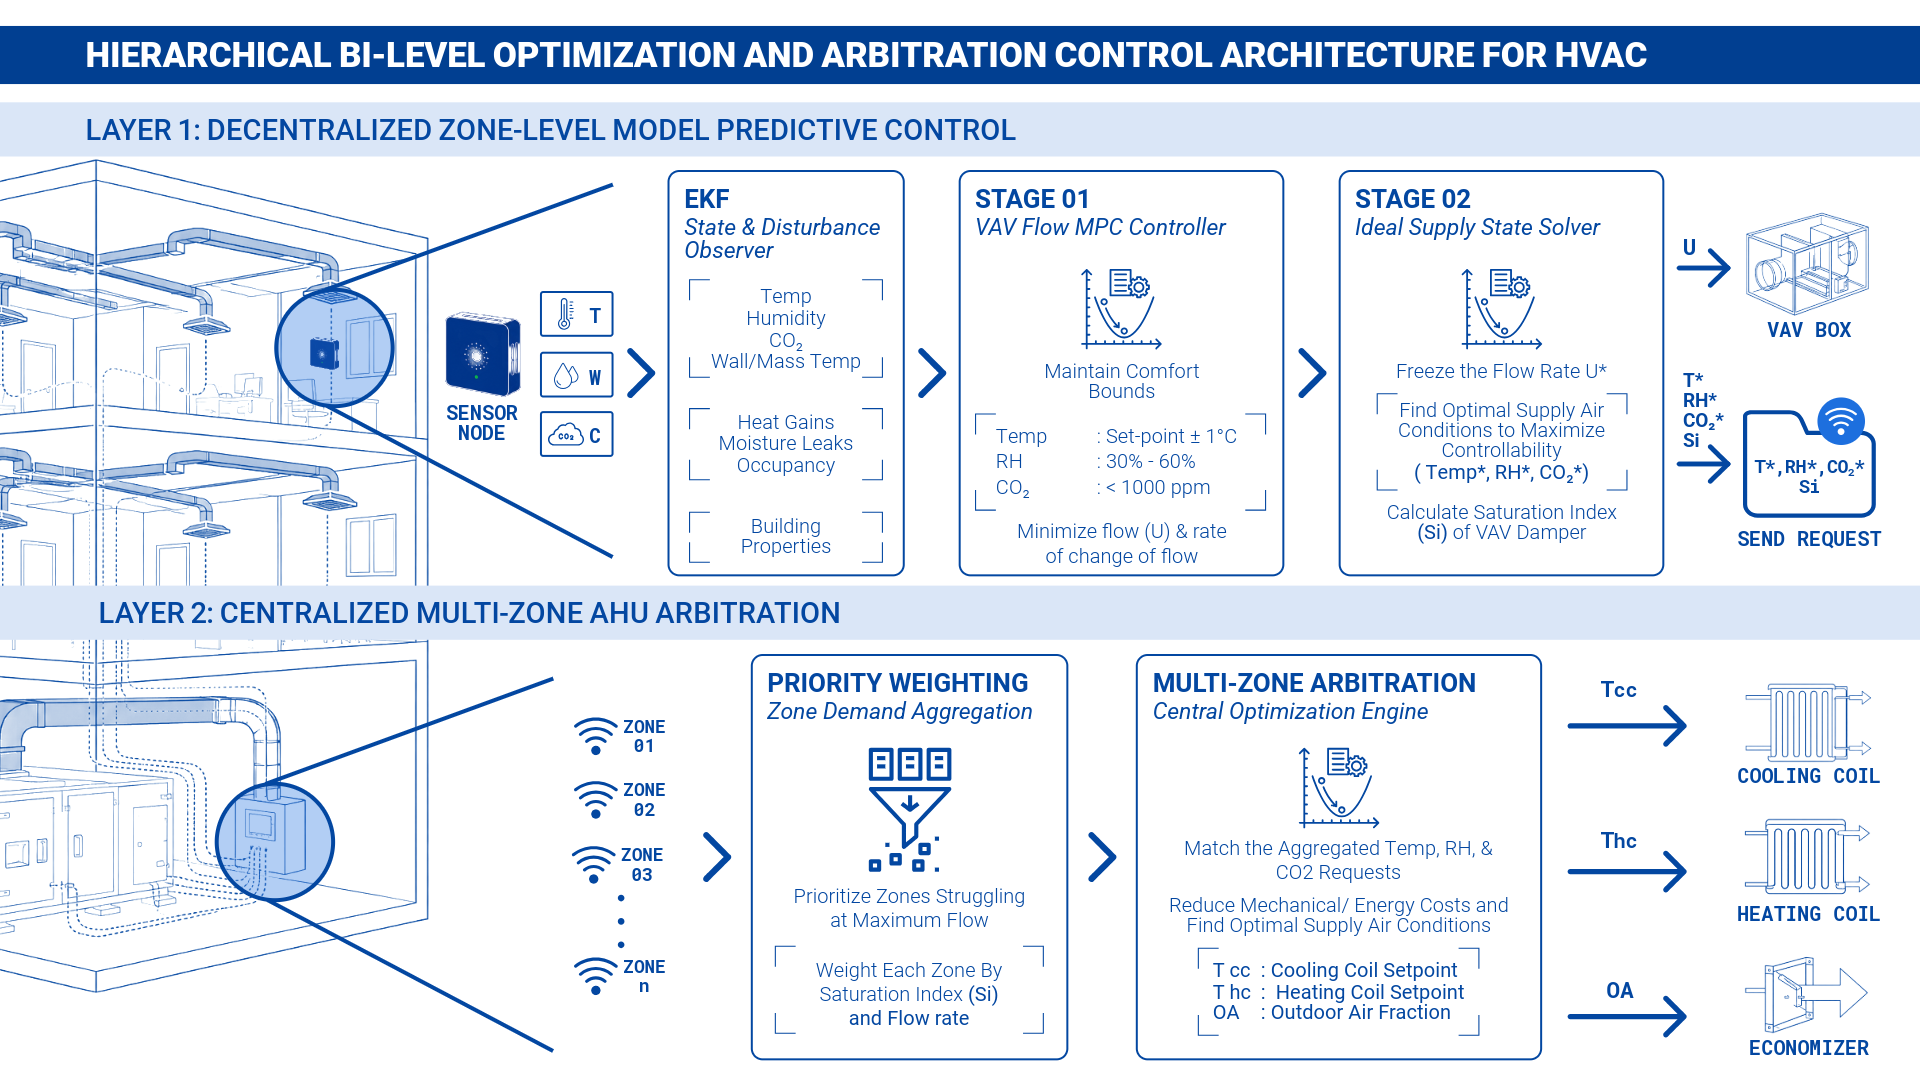
\includegraphics[width=\textwidth]{images/fig_architecture_overview.png}
		\caption{Hierarchical Bi-Level Optimization and Arbitration Control Architecture for Multi-Zone HVAC}
		\label{fig:architecture_overview}
	\end{figure}
	
	\newpage
	\subsection{Dynamic System Derivation}
	\label{sec:rc-model}

	
	\subsubsection{Fundamental Electrical Analogy}
	
	The thermal and mass transfer dynamics of each zone are modelled using an
	analogy with electrical RC circuits. In this analogy, temperature acts as the
	driving potential, heat flow represents the transport rate, thermal resistance
	represents resistance to heat transfer, and thermal capacitance represents heat
	storage. The same approach is used for moisture and CO$_2$, where
	humidity ratio and concentration act as the driving potentials.
	
	The purpose of the \textit{xR2C} model is not to produce fundamentally
	different physical equations from standard thermal and mass-transfer models.
	Instead, it retains the dominant zone dynamics while reducing unnecessary
	spatial detail and separating the important fast and slow dynamics. This gives
	a lower-order, control-oriented model that is easier to estimate, linearise,
	and use repeatedly within the MPC. The model therefore provides a practical
	balance between physical representation and computational cost.
	
	

	\subsubsection{Single-Zone Governing Equations}

	
	The \textbf{2R2C} network represents each zone using two thermal storage
	nodes, the indoor air node and the building mass node. The mass node represents
	the walls, floor, ceiling, furniture, and other solid elements with significant
	thermal mass. The two nodes represent different time scales of the zone response. The air
	node has a relatively small thermal capacity and therefore responds quickly to
	changes in outdoor conditions, internal gains, and supply air. This represents
	the \textit{fast dynamics}. The building mass has a larger thermal capacity and
	changes temperature more slowly, representing the \textit{slow dynamics} and
	thermal inertia of the building.
	
	The resistances represent the main paths of heat transfer. $R_{\mathrm{env}}$
	represents the thermal resistance between the outdoor environment and the
	indoor air, while $R_{\mathrm{int}}$ represents the thermal resistance between
	the indoor air and the building mass. The capacitances
	$C_{\mathrm{air}}$ and $C_{\mathrm{mass}}$ represent the heat-storage
	capacity of the air and building mass, respectively.
	
	\noindent{For a single zone, the governing equations are,}
	
	\noindent \textit{Air node:}
	\begin{equation}
		C_{\mathrm{air}} \frac{dT_{\mathrm{in}}}{dt}
		=
		\frac{T_{\mathrm{out}} - T_{\mathrm{in}}}{R_{\mathrm{env}}}
		+
		\frac{T_m - T_{\mathrm{in}}}{R_{\mathrm{int}}}
		+
		Q_{\mathrm{int}}
		+
		Q_{\mathrm{solar,conv}}
		+
		Q_{\mathrm{inf}}
		+
		\rho_{\mathrm{air}} c_p \dot{V}_s
		\left(T_s - T_{\mathrm{in}}\right)
		\label{eq:air_node_single}
	\end{equation}
	
	\noindent \textit{Mass node:}
	\begin{equation}
		C_{\mathrm{mass}} \frac{dT_m}{dt}
		=
		\frac{T_{\mathrm{in}} - T_m}{R_{\mathrm{int}}}
		+
		Q_{\mathrm{solar,rad}}
		\label{eq:mass_node_single}
	\end{equation}
	
	\noindent {Humidity and CO$_2$ are represented using single-node mass
		balances. A separate solid storage node is not included for humidity since it is negligible, similarly
		CO$_2$ is represented as a single-node concentration balance.
		The corresponding equations are,}
	
	\begin{equation}
		M_{\mathrm{air}} \frac{dW_{\mathrm{in}}}{dt}
		=
		G_{w,\mathrm{int}}
		+
		\dot{m}_{\mathrm{inf}}
		(W_{\mathrm{out}} - W_{\mathrm{in}})
		+
		\dot{m}_{s}
		(W_s - W_{\mathrm{in}})
		\label{eq:humidity_single}
	\end{equation}
	
	\begin{equation}
		V_{\mathrm{room}} \frac{dC_{\mathrm{in}}}{dt}
		=
		G_{\mathrm{co2,int}}
		+
		\dot{V}_{\mathrm{inf}}
		(C_{\mathrm{out}} - C_{\mathrm{in}})
		+
		\dot{V}_{s}
		(C_s - C_{\mathrm{in}})
		\label{eq:co2_single}
	\end{equation}
	
	

	\subsubsection{Model Simplification}

	
	The full physical model contains several inputs and interactions that are difficult to measure directly during operation. For control, these terms are simplified into known estimates and lumped disturbances. This reduces the number of model inputs while retaining their main effect on the zone dynamics.
	
	\noindent\textbf{Heuristic Estimation from Occupancy}
	
	If the occupant count $N_{\mathrm{occ}}$ is available from scheduling or from the EKF estimate, the internal generation terms are estimated using standard occupancy generation rates,
	
	\begin{equation}
		Q_{\mathrm{int},i}
		\approx
		N_{\mathrm{occ},i} q_{\mathrm{person}}
		+
		Q_{\mathrm{equip}},
		\qquad
		G_{w,\mathrm{int},i}
		\approx
		N_{\mathrm{occ},i} g_{w,\mathrm{person}},
		\qquad
		G_{\mathrm{co2,int},i}
		\approx
		N_{\mathrm{occ},i} g_{\mathrm{co2,person}}
		\label{eq:heuristic_gen}
	\end{equation}
	
	
	\noindent\textbf{Lumped Disturbance Representation}
	
	Several effects cannot be measured reliably or are difficult to model
	explicitly, such as  solar gains, infiltration, inter-zone exchange, and
	unmodelled heat and mass transfer. These effects are grouped into three
	lumped disturbance variables for each zone. The EKF estimates these
	disturbances during operation.
	
	\begin{align}
		d_{T,i}
		&=
		Q_{\mathrm{int},i}
		+
		Q_{\mathrm{solar,conv},i}
		+
		Q_{\mathrm{inf},i}
		+
		\text{unmodelled conduction}
		\label{eq:dT}
		\\
		d_{W,i}
		&=
		\dot{m}_{\mathrm{inf},i}
		(W_{\mathrm{out}}-W_{\mathrm{in},i})
		+
		\text{unmodelled moisture transfer}
		\label{eq:dW}
		\\
		d_{C,i}
		&=
		\dot{V}_{\mathrm{inf},i}
		(C_{\mathrm{out}}-C_{\mathrm{in},i})
		+
		\text{unmodelled CO$_2$ transfer}
		\label{eq:dC}
	\end{align}
	
	
	\noindent\textbf{Simplified Operating Equations}
	
	The occupancy estimates and lumped disturbances are then substituted into
	the zone model. Using
	
	\begin{equation}
		M_{\mathrm{air}} = \frac{C_{\mathrm{air}}}{c_p},
		\qquad
		V_{\mathrm{room}}
		=
		\frac{C_{\mathrm{air}}}{\rho_{\mathrm{air}}c_p},
	\end{equation}
	
	the model is reduced to the four states used by the controller. The zone
	index $i$ is omitted for compactness, and $u=\dot{V}_s$ denotes the VAV
	volumetric flow rate.
	
	\begin{align}
		\dot{T}_{\mathrm{in}}
		&=
		\frac{1}{C_{\mathrm{air}}}
		\left[
		\frac{T_{\mathrm{out}}-T_{\mathrm{in}}}{R_{\mathrm{ext}}}
		+
		\frac{T_m-T_{\mathrm{in}}}{R_{\mathrm{int}}}
		+
		N_{\mathrm{occ}}q_{\mathrm{per}}
		+
		\rho_{\mathrm{air}}c_pu(T_s-T_{\mathrm{in}})
		+
		d_T
		\right]
		\label{eq:simplified_T}
		\\
		\dot{T}_m
		&=
		\frac{1}{C_{\mathrm{mass}}}
		\left[
		\frac{T_{\mathrm{in}}-T_m}{R_{\mathrm{int}}}\right]
		\label{eq:simplified_Tm}
		\\
		\dot{W}_{\mathrm{in}}
		&=
		\frac{c_p}{C_{\mathrm{air}}}
		\left[
		N_{\mathrm{occ}}g_{w,\mathrm{per}}
		+
		\rho_{\mathrm{air}}u(W_s-W_{\mathrm{in}})
		+
		d_W
		\right]
		\label{eq:simplified_W}
		\\
		\dot{C}_{\mathrm{in}}
		&=
		\frac{\rho_{\mathrm{air}}c_p}{C_{\mathrm{air}}}
		\left[
		N_{\mathrm{occ}}g_{\mathrm{co2,per}}
		+
		u(C_s-C_{\mathrm{in}})
		+
		d_C
		\right]
		\label{eq:simplified_C}\\
	\end{align}
	\newpage
	\noindent\textbf{State, Measurement, and Input Representation}
	
	The resulting control-oriented state vector is
	
	\begin{equation}
		x =
		\begin{bmatrix}
			T_{\mathrm{in}} &
			T_m &
			W_{\mathrm{in}} &
			C_{\mathrm{in}}
		\end{bmatrix}^{T}
	\end{equation}
	
	with measured outputs
	
	\begin{equation}
		y =
		\begin{bmatrix}
			T_{\mathrm{in}} &
			W_{\mathrm{in}} &
			C_{\mathrm{in}}
		\end{bmatrix}^{T}
	\end{equation}
	
	The control input is the VAV supply-air volumetric flow rate,
	
	\begin{equation}
		u = \dot{V}_s.
		\label{eq:state_vectors}
	\end{equation}
	
	The mass temperature $T_m$ is not directly measured by the available zone
	sensors and is therefore treated as a hidden state. It is estimated online
	using the EKF.
	
	\newpage
	\subsection{State Estimation via the Extended Kalman Filter (EKF)}
	\label{sec:ekf}

	The zone controller uses an Extended Kalman Filter (EKF) as a combined state observer, disturbance observer, and online parameter estimator. Rather than estimating only the directly measured zone variables, the filter maintains an augmented representation of the zone dynamics containing physical states, unmeasured disturbances, occupancy, and uncertain model parameters. This allows the controller to operate using a continuously updated representation of the zone condition and its underlying thermal behaviour.
	
	\subsubsection{Augmented State Vector}
	
	The EKF operates on the following 11-element augmented state vector:
\begin{equation}
	x_a =
	\begin{bmatrix}
		T_{\mathrm{in}} \\
		T_m \\
		W_{\mathrm{in}} \\
		C_{\mathrm{in}} \\
		d_T \\
		d_W \\
		N_{\mathrm{occ}} \\
		\alpha_{\mathrm{ext}} \\
		\alpha_{\mathrm{int}} \\
		\beta_{\mathrm{air}} \\
		\beta_{\mathrm{mass}}
	\end{bmatrix}_{11\times1}
	\label{eq:augmented_state}
\end{equation}
	
	where
	\begin{equation}
		\alpha_{\mathrm{ext}}=\frac{1}{R_{\mathrm{ext}}},
		\qquad
		\alpha_{\mathrm{int}}=\frac{1}{R_{\mathrm{int}}},
		\qquad
		\beta_{\mathrm{air}}=\frac{1}{C_{\mathrm{air}}},
		\qquad
		\beta_{\mathrm{mass}}=\frac{1}{C_{\mathrm{mass}}}.
	\end{equation}
	
	The augmented state has three distinct functions within the estimator.
	
	\subsubsection{Sensor Fusion and Hidden-State Estimation}
	
	The first four states, $\left[ T_{\mathrm{in}}, T_m, W_{\mathrm{in}}, C_{\mathrm{in}} \right]^T$, represent the physical condition of the zone. The available sensors directly measure indoor air temperature, humidity ratio, and $CO_2$ concentration, while the thermal mass temperature $T_m$ is not directly measured. The EKF therefore combines the three measured variables with the dynamic model to estimate the hidden thermal-mass state.
	
	This provides a state estimate that is more informative than the raw sensor measurements alone. In particular, $T_m$ captures the slower thermal response of the building fabric and furniture, allowing the controller to distinguish short-term air-temperature changes from the underlying thermal condition of the zone. The measurement model therefore observes only the three air-side states,
	\begin{equation}
		y =
		\begin{bmatrix}
			T_{\mathrm{in}} \\
			W_{\mathrm{in}} \\
			C_{\mathrm{in}}
		\end{bmatrix},
		\qquad
		H =
		\begin{bmatrix}
			1&0&0&0&0&0&0&0&0&0&0 \\
			0&0&1&0&0&0&0&0&0&0&0 \\
			0&0&0&1&0&0&0&0&0&0&0
		\end{bmatrix}.
		\label{eq:H_matrix}
	\end{equation}
	
	\subsubsection{Disturbance and Occupancy Observation}
	
	The next three states, $\left[ d_T, d_W, N_{\mathrm{occ}} \right]^T$, act as online disturbance estimates. Instead of attempting to model every unmeasured source of variation explicitly, the dominant unknown effects are represented by lumped disturbance states.
	
	The thermal disturbance $d_T$ captures unmodelled sensible heat gains and losses, including effects such as solar gains, infiltration, inter-zone interactions, and other discrepancies between the simplified model and the actual zone. Similarly, $d_W$ represents unmodelled moisture sources and sinks.	Occupancy is treated separately because it provides a useful common explanatory variable across multiple physical processes. In particular, the same occupancy estimate can contribute simultaneously to sensible heat generation and moisture generation through
	\begin{equation}
		Q_{\mathrm{occ}} \approx N_{\mathrm{occ}}q_{\mathrm{per}},
		\qquad
		G_{w,\mathrm{occ}} \approx N_{\mathrm{occ}}g_{w,\mathrm{per}}.
	\end{equation}
	Thus, rather than estimating independent unknown disturbances for every internal process, occupancy provides a physically interpretable latent variable that links thermal and moisture generation. This coupling provides the estimator with additional structure and can produce more consistent estimates when the available measurements do not directly reveal the underlying internal loads.
	
	The disturbance and occupancy states are modelled using a slowly decaying mean-reverting process, 	where $\tau$ is selected to allow persistent disturbances to be tracked while preventing their estimates from accumulating indefinitely when the measurements provide insufficient correction.
	\begin{equation}
		\dot d_T=-\frac{d_T}{\tau},
		\qquad
		\dot d_W=-\frac{d_W}{\tau},
		\qquad
		\dot N_{\mathrm{occ}}=-\frac{N_{\mathrm{occ}}}{\tau},
		\label{eq:OU_dynamics}
	\end{equation}
	
	\subsubsection{Online Physical-Parameter Estimation}
	
	The final four states, $\left[ \alpha_{\mathrm{ext}}, \alpha_{\mathrm{int}}, \beta_{\mathrm{air}}, \beta_{\mathrm{mass}} \right]^T$, represent uncertain physical parameters of the thermal model. These correspond respectively to the external and internal thermal conductances and the inverse thermal capacitances of the air and thermal-mass nodes.	A reasonably good initial estimate is provided from the available building information, but the parameters are not treated as permanently fixed. Instead, the EKF allows them to adapt gradually as new measurements become available. Small process-noise levels are assigned to these states so that they evolve much more slowly than the physical and disturbance states.
	
	This provides an online system-identification capability. The estimated parameters can therefore adapt to gradual changes in effective zone behaviour caused by changes in operating conditions, occupancy patterns, equipment operation, or other time-varying characteristics that are not fully represented by the nominal model. The resulting model is consequently not a fixed physics model, but an adaptive representation continuously refined from measured zone behaviour.
	
	\subsubsection{EKF Prediction and Measurement Correction}
	
	Because the model is nonlinear, the continuous dynamics are locally linearised about the current estimated operating point using the Jacobian. The resulting local model is discretised over the simulation timestep and used in the standard EKF prediction and correction procedure.
	\begin{equation}
		F =
		\frac{\partial f}{\partial x_a}.
	\end{equation}

	To maintain numerical stability when the control loop interval is larger than the natural time scale of the zone dynamics, the prediction step is internally sub-stepped. The state and covariance are propagated through the smaller intervals, after which a single measurement correction is applied using the available $T_{\mathrm{in}}$, $W_{\mathrm{in}}$, and $C_{\mathrm{in}}$ measurements.
	
	\subsubsection{EKF Tuning}
	
	The process and measurement covariance matrices are diagonal and are tuned according to the expected rate of variation and confidence associated with each state. The tuning is intentionally hierarchical rather than treating all states identically.
	The resulting tuning hierarchy gives the estimator different levels of freedom. Disturbance and occupancy states are permitted to respond to relatively rapid changes, measured physical states are corrected strongly by reliable sensor information, and the structural parameters are deliberately constrained to evolve slowly. This prevents the filter from using parameter adaptation to explain short-term disturbances while still allowing the estimated model to evolve as the effective thermal behaviour of the zone changes over time.

	
	\begin{table}[ht]
		\centering
		\caption{EKF process covariance tuning strategy.}
		\label{tab:EKF_state_covariances}
		\begin{tabular}{lll}
			\toprule
			\textbf{State} & \textbf{Symbol} & \textbf{Tuning Intent} \\
			\midrule
			Indoor air temperature
			& $T_{\mathrm{in}}$
			& Track core physical dynamics \\
			
			Thermal mass temperature
			& $T_m$
			& Allow slow hidden-state evolution \\
			
			Humidity ratio
			& $W_{\mathrm{in}}$
			& Track measured moisture dynamics \\
			
			CO$_2$ concentration
			& $C_{\mathrm{in}}$
			& Track measured IAQ dynamics \\
			
			Thermal disturbance
			& $d_T$
			& Allow fast disturbance changes \\
			
			Latent disturbance
			& $d_W$
			& Allow fast moisture-load changes \\
			
			Occupancy
			& $N_{\mathrm{occ}}$
			& Allow relatively fast occupancy changes \\
			
			Envelope conductance
			& $\alpha_{\mathrm{ext}}$
			& Allow very slow physical adaptation \\
			
			Internal conductance
			& $\alpha_{\mathrm{int}}$
			& Allow very slow physical adaptation \\
			
			Air capacitance inverse
			& $\beta_{\mathrm{air}}$
			& Allow very slow physical adaptation \\
			
			Mass capacitance inverse
			& $\beta_{\mathrm{mass}}$
			& Allow very slow physical adaptation \\
			
			\bottomrule
		\end{tabular}
	\end{table}
	
	Overall, the resulting estimator is more than a conventional EKF applied to a fixed thermal model. It combines sensor fusion and hidden-state estimation, online disturbance and occupancy observation, and slow online parameter identification within a single estimation framework. This adaptive state representation is subsequently used by the zone MPC to predict the effect of VAV actuation using the current estimated condition, disturbances, and physical characteristics of the zone.
%	\begin{table}[ht]
%		\centering
%		\caption{EKF measurement covariance tuning strategy.}
%		\label{tab:EKF_measurement_covariances}
%		\begin{tabular}{lll}
%			\toprule
%			\textbf{Measurement} & \textbf{Symbol} & \textbf{Tuning Intent} \\
%			\midrule
%			Temperature measurement
%			& $T_{\mathrm{in}}$
%			& Trust sensor reading according to sensor accuracy \\
%			
%			Humidity measurement
%			& $W_{\mathrm{in}}$
%			& Trust sensor reading according to sensor accuracy \\
%			
%			CO$_2$ measurement
%			& $C_{\mathrm{in}}$
%			& Trust sensor reading according to sensor accuracy \\
%			
%			\bottomrule
%		\end{tabular}
%	\end{table}
	

% ----------------------------------------------------------


	\newpage
	
	\subsection{Layer 1 - Zone Controller: Comfort- and IAQ-Constrained MPC}
	\label{sec:stage1}
	% ----------------------------------------------------------
	
	\begin{figure}[h!]
		\centering
		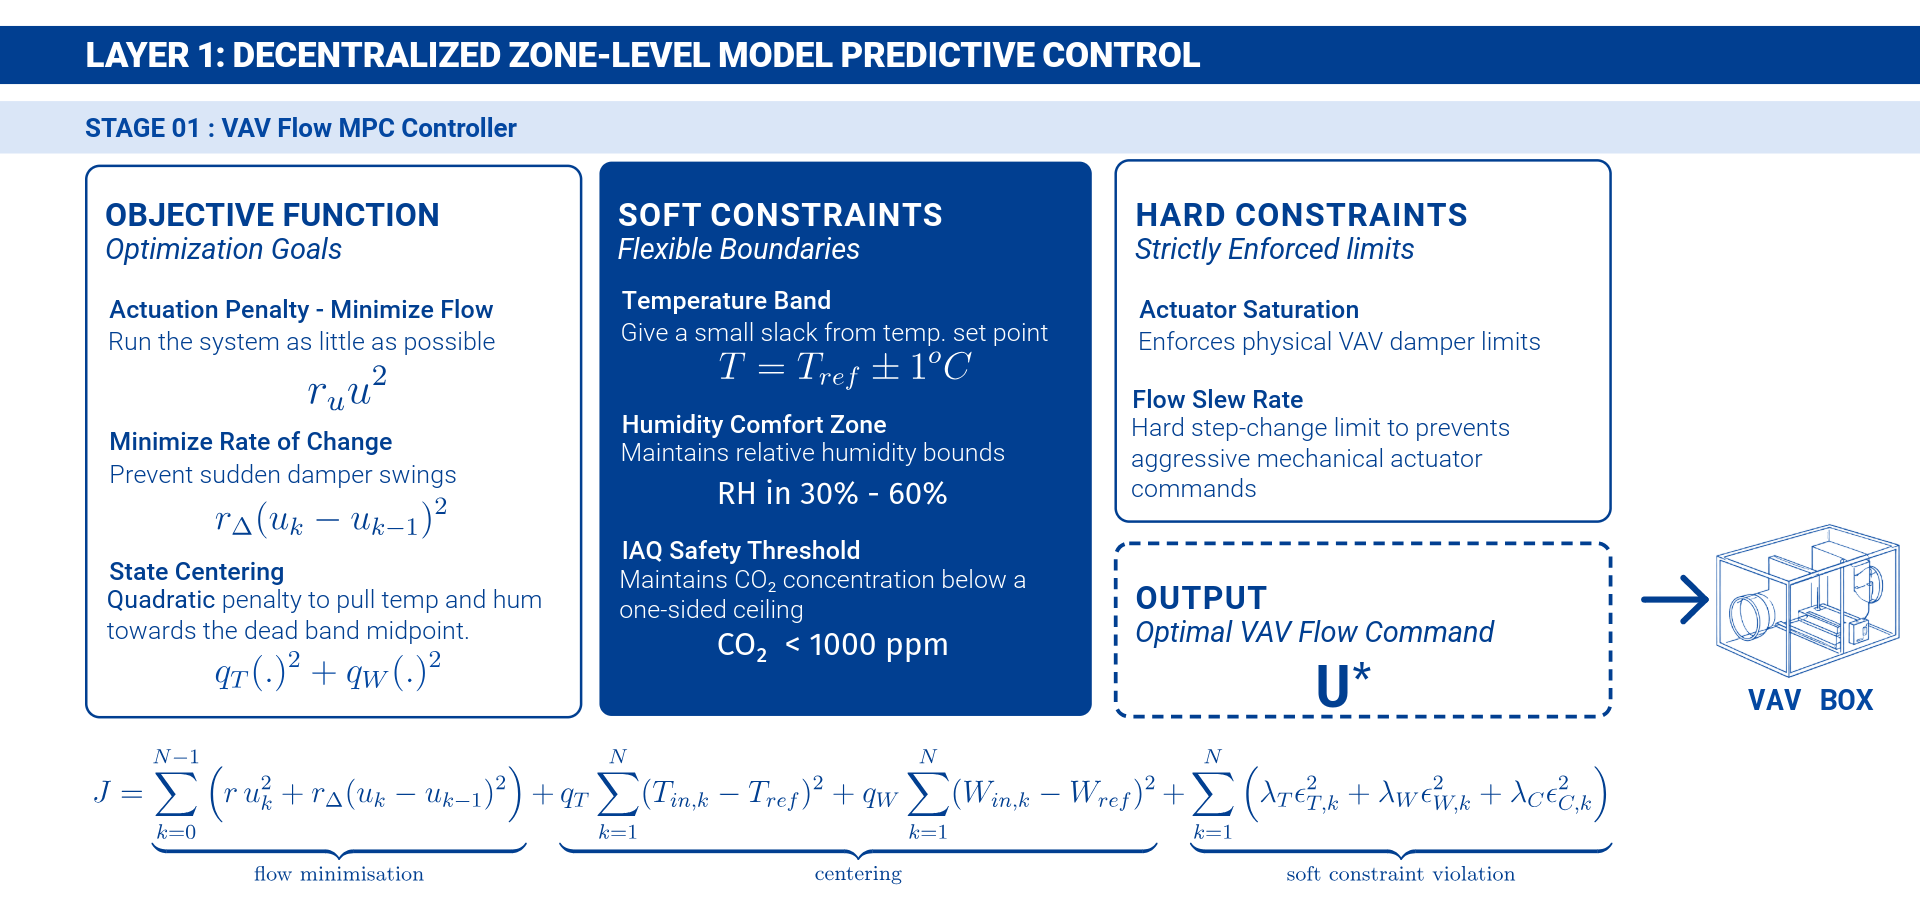
\includegraphics[width=1.0\textwidth]{images/fig_stage1_flow_mpc.png}
		\caption{Layer~1, Stage~1 - Comfort and IAQ constrained flow MPC}
		\label{fig:stage1_flow_mpc}
	\end{figure}
	
	\subsubsection{Control Philosophy}
	
	The first-stage Zone Controller determines the VAV airflow required to maintain acceptable indoor conditions. Rather than treating temperature, humidity, and CO$_2$ as conventional tracking variables with independent setpoints, the controller formulates them primarily as \textbf{soft constraints}. This allows the available airflow to be allocated according to the most critical zone condition at each timestep.
	
	Temperature remains associated with a user- or schedule-defined reference temperature $T_{\mathrm{ref}}$.  A small deadband is constructed around the reference, providing the zone with sufficient operating freedom to accommodate humidity and CO$_2$ requirements. Humidity is constrained to an acceptable range corresponding to prescribed relative-humidity limits, while the CO$_2$ concentration is constrained by an upper IAQ ceiling. These limits are derived from the adopted ASHRAE-based comfort and indoor-air-quality criteria. 
		
	\subsubsection{Comfort and IAQ Operating Regions}
	
	The allowable operating region is defined independently for the three controlled variables as illustrated in Figure~\ref{fig:comfort_zone}.	For temperature, the reference value provides the centre of a local comfort deadband,
	\begin{equation}
		T_{\min,\max} = T_{\mathrm{ref}} \pm \Delta T_{\mathrm{db}}
	\end{equation}
	
	For humidity, the controller does not use a fixed humidity-ratio reference. Instead, the allowable humidity ratio bounds are obtained from the corresponding relative  humidity limits at the predicted indoor temperature. This temperature dependent representation allows the humidity constraint to remain physically consistent with the psychrometric relationship between temperature, humidity ratio, and relative humidity,
	\begin{equation}
		W_{\min} = W(T_{\mathrm{in}},\, RH_{\min}), \qquad W_{\max} = W(T_{\mathrm{in}},\, RH_{\max}).
	\end{equation}
	
	CO$_2$ is formulated as a one sided IAQ constraint,
	\begin{equation}
		C_{\mathrm{in}} \le C_{\max}.
	\end{equation}
	
	The three individual bounds and their combined representation on a psychrometric chart are shown in Figure~\ref{fig:comfort_zone} while 	Table~\ref{tab:MPC_zone_limits} summarises the numerical values of all comfort and actuator limits applied in the Phase-1 MPC.
	
	\begin{figure}[ht]
		\centering
		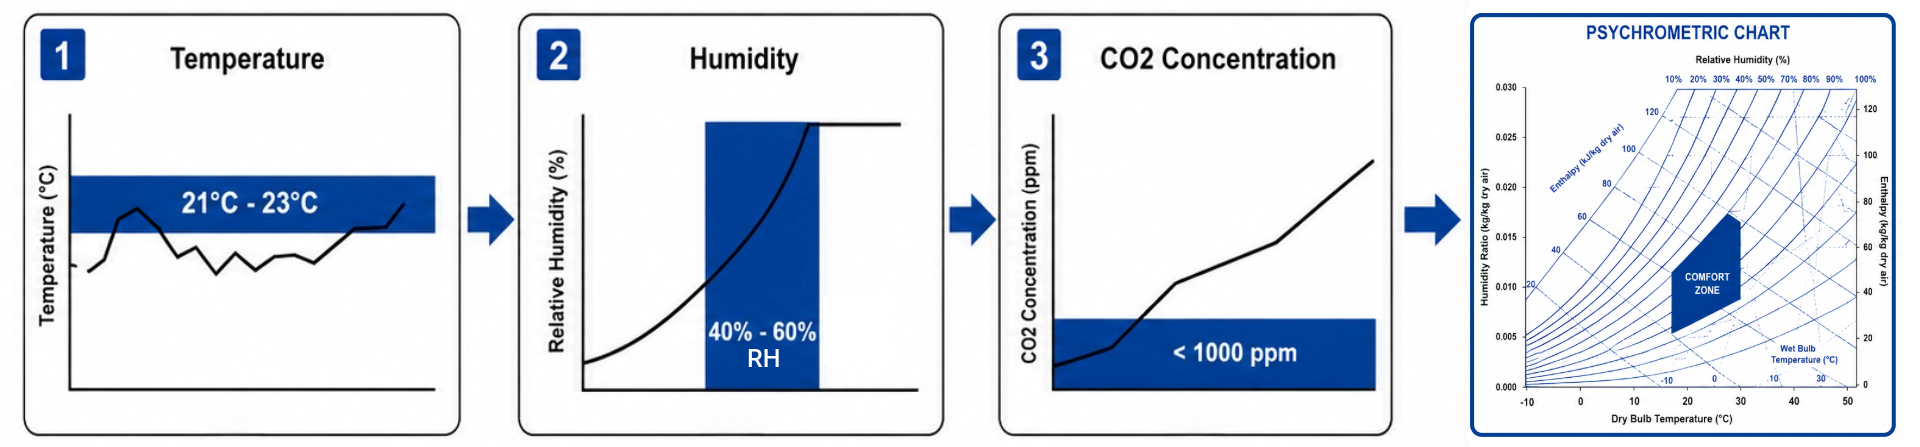
\includegraphics[width=\linewidth]{images/fig_comfort_zone.png}
		\caption{Comfort and IAQ operating regions}
		\label{fig:comfort_zone}
	\end{figure}

	
	\begin{table}[ht]
		\centering
		\caption{Zone comfort and actuator limits applied in the Phase-1 MPC.}
		\label{tab:MPC_zone_limits}
		\begin{tabular}{llll}
			\toprule
			\textbf{Variable} & \textbf{Min} & \textbf{Max} & \textbf{Notes} \\
			\midrule
			$T_{\mathrm{in}}$
			& $T_{\mathrm{ref}} - 1\,^{\circ}\mathrm{C}$
			& $T_{\mathrm{ref}} + 1\,^{\circ}\mathrm{C}$
			& Deadband around per-zone temperature reference \\[4pt]
			$W_{\mathrm{in}}$
			& $W(T_{\mathrm{in}},\,RH=30\%)$
			& $W(T_{\mathrm{in}},\,RH=60\%)$
			& Psychrometric conversion at predicted temperature \\[4pt]
			$C_{\mathrm{in}}$
			& ---
			& $1000\,\mathrm{ppm}$
			& One-sided IAQ ceiling \\[4pt]
			$u$
			& $0.05\,\mathrm{m^3/s}$
			& $2.0\,\mathrm{m^3/s}$
			& Hard VAV actuator limits \\
			\bottomrule
		\end{tabular}
	\end{table}
	
	
	\subsubsection{Objective Function}
	
	The MPC objective is formulated around three complementary goals, minimise the required airflow, avoid unnecessary changes in airflow, and discourage violations of the comfort and IAQ operating regions.
	
	\begin{equation}
		\begin{aligned}
			\min J ={}&
			\underbrace{
				\sum_{k=0}^{N-1}
				\left[
				r\,u_k^2+
				r_{\Delta}(u_k-u_{k-1})^2
				\right] 
			}_{\substack{\text{actuation}\\\text{minimisation}}} 
			\quad+
			\\[6pt]
			&
			\underbrace{
				q_T\sum_{k=1}^{N}
				(T_{\mathrm{in},k}-T_{\mathrm{ref}})^2
				+
				q_W\sum_{k=1}^{N}
				(W_{\mathrm{in},k}-W_{\mathrm{ref}})^2
			}_{\substack{\text{deadband}\\\text{centering}}}
			\quad+
			\\[6pt]
			&
			\underbrace{
				\sum_{k=1}^{N}
				\left[
				\lambda_T\epsilon_{T,k}^2+
				\lambda_W\epsilon_{W,k}^2+
				\lambda_C\epsilon_{C,k}^2
				\right]
			}_{\substack{\text{soft comfort and}\\\text{IAQ violations}}}.
		\end{aligned}
		\label{eq:MPC_objective}
	\end{equation}
	
	
	where
	
	\begin{equation}
		W_{\mathrm{ref}} = 	\frac{W_{\max}+W_{\min}}{2}
	\end{equation}
	
	The first term penalises absolute VAV flow and therefore encourages the controller to satisfy the zone requirements with the lowest possible airflow. The second term penalises rapid changes in the VAV command. This discourages unnecessary actuator movement and produces smoother airflow trajectories.
	
	The third term represents the central mechanism of the controller. Slack variables $\epsilon_T$, $\epsilon_W$, and $\epsilon_C$ allow the predicted comfort and IAQ limits to be violated when the available actuation is insufficient to satisfy all constraints simultaneously.  The temperature and humidity centering terms have a different role from the soft constraints. They do not define additional comfort requirements. Instead, they provide a preferred location within the feasible region. Temperature is gently pulled toward $T_{\mathrm{ref}}$, while humidity is biased toward the middle of its allowable range. This prevents the predicted trajectory from repeatedly operating near the edge of the deadband, where a small disturbance could immediately require a large corrective airflow. CO$_2$ is not given a centering term because its control objective is primarily to remain below the IAQ ceiling rather than to track an arbitrary concentration.
	
	
	\subsubsection{Soft Constraints}
		\noindent{The soft constraint penalty hierarchy is selected as,}
	
	\begin{equation}
		\lambda_T > \lambda_W > \lambda_C >  r 
	\end{equation}
	
	where $\lambda_T$, $\lambda_W$, and $\lambda_C$ penalise violations of the temperature, humidity, and CO$_2$ limits, respectively, while $r$ penalises airflow. The controller is deliberately willing to increase airflow when necessary to protect zone conditions. At the same time, the hierarchy establishes a priority among competing requirements.
	\subsubsection{Hard Actuator Constraints}
	
	While comfort and IAQ requirements are soft, the physical limitations of the VAV actuator are enforced as hard constraints. The predicted airflow and its rate of change must satisfy
	
	\begin{equation}
		u_{\min}\leq u_k\leq u_{\max},
	\end{equation}
	
	\begin{equation}
		-\Delta u_{\max}
		\leq
		u_k-u_{k-1}
		\leq
		\Delta u_{\max}.
	\end{equation}
	
	These constraints are not softened because violating them would result to commanding a physically unavailable airflow or an unrealistically sudden actuator movement. The hard slew rate constraint also provides protection against large flow changes when the soft comfort and IAQ constraints become active during strong disturbances. Therefore, MPC separates \textbf{physical feasibility} from \textbf{environmental acceptability}. 
	
	\subsubsection{Prediction, MPC Formulation and Tuning Strategy}
	
	At every control timestep, the EKF provides the current estimate of the zone state and the associated disturbance states. The nonlinear zone model is then locally linearised around the current operating point and discretised for prediction over the MPC horizon. The resulting linear prediction model maps the candidate VAV flow sequence to predicted trajectories of,
	
	\[
	T_{\mathrm{in},1:N},\qquad
	W_{\mathrm{in},1:N},\qquad
	C_{\mathrm{in},1:N}.
	\]
	These trajectories are used directly to construct the temperature, humidity, and CO$_2$ soft constraints. The optimisation problem is then assembled as a quadratic program with the VAV flow sequence and the corresponding slack variables as decision variables.
	
	\subsubsection{Tuning Strategy}
	
	The tuning parameters are selected according to their control role.
	The overall tuning objective is  hierarchical \textbf{maintain acceptable indoor conditions first, minimise airflow second, and minimise unnecessary actuator movement}. The centering terms provide additional robustness within the allowable region without replacing the constraint-based nature of the controller.
	
	\begin{table}[ht]
		\centering
		\caption{Phase-1 MPC tuning parameters and their control rationale.}
		\label{tab:MPC_tuning}
		\begin{tabular}{p{0.12\textwidth}p{0.88\textwidth}}
			\toprule
			\textbf{Parameter} & \textbf{Control rationale} \\
			\midrule
			
			$N$
			& Prediction horizon . \\[2pt]
			
			$r$
			& Small relative penalty on absolute VAV flow, encourages minimum  effort without overriding comfort or IAQ requirements. \\[2pt]
			
			$r_\Delta$
			& Penalises changes in VAV flow and promotes smooth actuator operation. \\[2pt]
			
			$\lambda_T$
			& High penalty on temperature bound violations, establishes temperature as the highest-priority soft constraint. \\[2pt]
			
			$\lambda_W$
			& High penalty on humidity bound violations, lower than temperature but  larger than the actuation cost. \\[2pt]
			
			$\lambda_C$
			& Penalty on CO$_2$ ceiling violation, ensures IAQ is actively maintained while allowing limited transient violation when required by actuator or competing constraints. \\[2pt]
			
			$q_T$
			& Moderate centering weight that keeps the predicted temperature near the specified reference without converting the deadband controller into a strict tracking controller. \\[2pt]
			
			$q_W$
			& Centering weight that biases humidity toward the middle of its acceptable range and provides margin against approaching either RH boundary. \\[2pt]
			
			$\Delta u_{\max}$
			& Hard rate limit selected to prevent abrupt VAV commands and maintain physically realistic actuator behaviour. \\
			
			\bottomrule
		\end{tabular}
	\end{table}

	\newpage

	% ----------------------------------------------------------
	\subsection{Layer 1 - Zone Controller: Ideal Supply State Solver}
	\label{sec:stage2}
	% ----------------------------------------------------------
	
	\begin{figure}[h!]
		\centering
		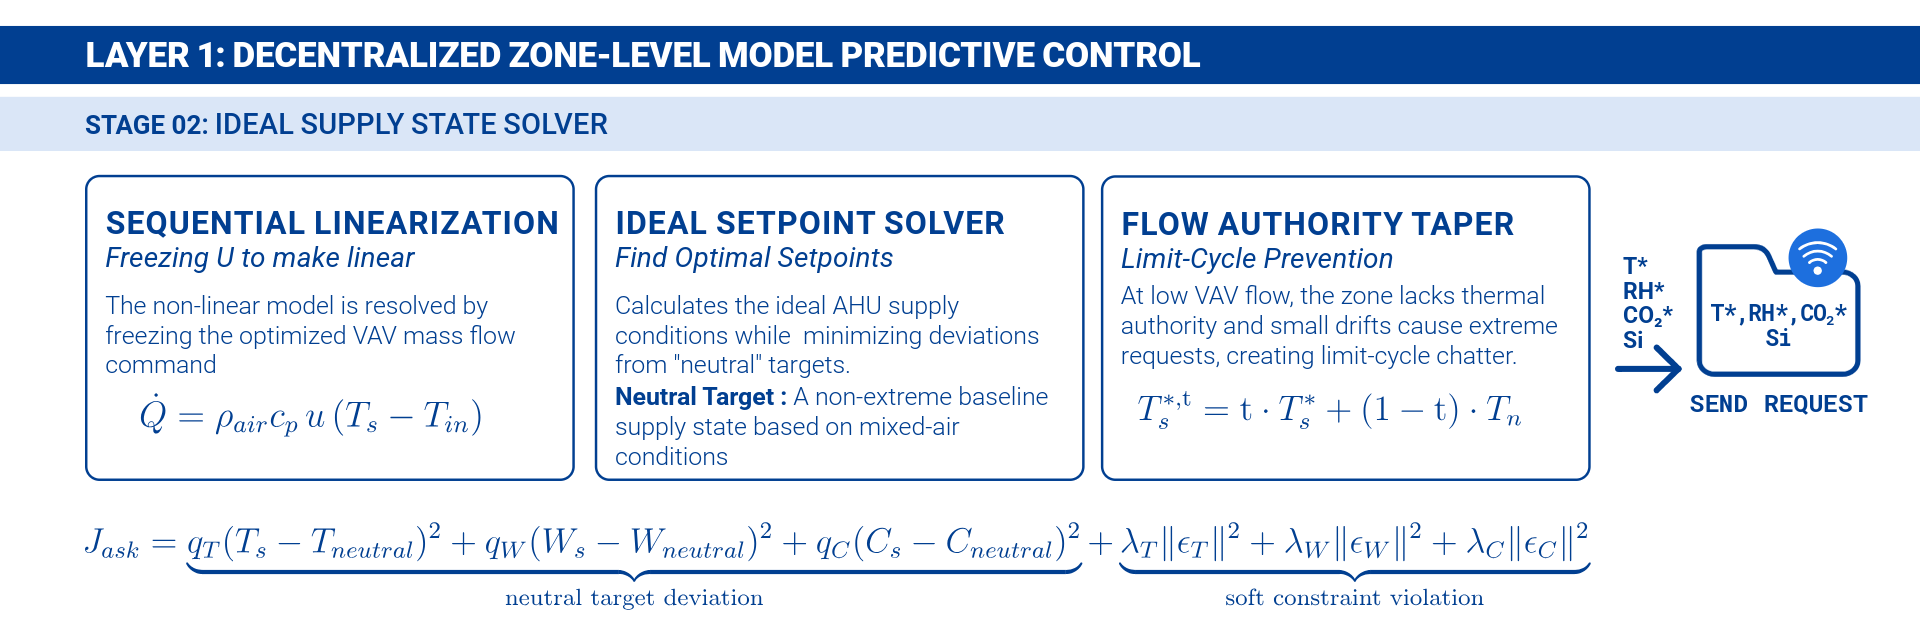
\includegraphics[width=1.0\textwidth]{images/fig_stage2_ideal_ask.png}
		\caption{Layer~1, Stage~2 -- the ideal-ask solver.}
		\label{fig:stage2_ideal_ask}
	\end{figure}
	
	\subsubsection{Sequential Linearisation and Supply-State Optimisation}
	
	Stage~1 determines the VAV flow required to maintain the zone within its temperature, humidity, and CO$_2$ limits. However, the resulting flow command alone does not determine how the available supply air should be conditioned. The supply air temperature, humidity ratio, and CO$_2$ concentration must also be selected to provide the required zone response.	The zone dynamics contain bilinear terms between the VAV flow and the supply air state. For example, the sensible cooling or heating contribution can be expressed as
	\[
	\dot{Q}_{s}
	=
	\rho_{\mathrm{air}}c_p u
	\left(T_s-T_{\mathrm{in}}\right)
	\]
	
	which couples the flow command $u$ with the supply temperature $T_s$. Simultaneously optimising both variables would therefore introduce a non-convex optimisation problem. 	The controller resolves this coupling through \textbf{sequential linearisation}. The two control decisions are separated into two phases.
	
	\begin{enumerate}
		\item \textbf{Stage~1 -- Flow optimisation:} the current supply-air state is treated as a known operating condition, and the MPC determines the minimum VAV flow required to maintain the zone comfort and IAQ constraints.
		
		\item \textbf{Stage~2 -- Supply-state optimisation:} the resulting flow command $u_{\mathrm{cmd}}$ is fixed. With the flow no longer a decision variable, the bilinear coupling becomes linear with respect to the supply-air state
		\[
		Z =
		\begin{bmatrix}
			T_s & W_s & C_s
		\end{bmatrix}^{T}
		\]
	\end{enumerate}
	
	The controller can therefore solve a convex quadratic program to determine the preferred supply-air state. This sequential formulation preserves the computational advantages of a convex QP while allowing the controller to coordinate both the quantity of air delivered to the zone and the condition of that air.
	
	\subsubsection{Dynamic Neutral Supply Target}
	
	The Stage~2 optimisation requires a reference supply condition. Directly optimising the supply state without such a reference could produce unnecessarily aggressive requests, particularly when the zone has limited thermal or mass-flow authority. The neutral target is based on an estimate of the outdoor-air fraction in the current mixed-air condition. The fraction is estimated from the measured indoor, outdoor, and supply CO$_2$ concentrations. where $\hat{\gamma}$ represents the estimated fraction of outdoor air. 
	
	\begin{equation}
		\hat{\gamma}
		=
		\mathrm{clip}\!\left(
		\frac{C_{\mathrm{in}}-C_s}
		{C_{\mathrm{in}}-C_{\mathrm{out}}},
		0,1
		\right),
		\label{eq:gamma_estimate}
	\end{equation}

	
	\begin{align}
		T_{\mathrm{neutral}}
		&=
		\mathrm{clip}\!\left(
		\hat{\gamma}T_{\mathrm{out}}
		+
		(1-\hat{\gamma})T_{\mathrm{in}},
		T_{s,\min},T_{s,\max}
		\right),
		\\
		W_{\mathrm{neutral}}
		&=
		\mathrm{clip}\!\left(
		\hat{\gamma}W_{\mathrm{out}}
		+
		(1-\hat{\gamma})W_{\mathrm{in}},
		W_{s,\min},W_{s,\max}
		\right),
		\\
		C_{\mathrm{neutral}}
		&=C_{\mathrm{in}}.
		\label{eq:neutral_targets}
	\end{align}
	
	\subsubsection{Ideal State Solver Objective, Penalties, and Constraints}
	
	With the Stage~1 flow command fixed, Stage~2 determines the supply state that provides the required zone response while remaining as close as practical to the dynamic neutral condition. The objective is,
		
	\begin{equation}
		\begin{aligned}
			\min  J_{\mathrm{ask}}
			={}&
			\underbrace{
				q_T\left(T_s-T_{\mathrm{neutral}}\right)^2
				+
				q_W\left(W_s-W_{\mathrm{neutral}}\right)^2
				+
				q_C\left(C_s-C_{\mathrm{neutral}}\right)^2
			}_{\substack{\text{avoid deviation from neutral supply state}}}
			+
			\\[6pt]
			&
			\underbrace{
				\lambda_T\|\epsilon_T\|^2
				+
				\lambda_W\|\epsilon_W\|^2
				+
				\lambda_C\|\epsilon_C\|^2
			}_{\substack{\text{soft comfort and IAQ constraint violations}}}.
		\end{aligned}
		\label{eq:ask_objective}
	\end{equation}
	
	The first three terms penalise unnecessary deviation of the requested supply state from the dynamic neutral condition. They prevent the controller from requesting unnecessarily extreme supply conditions when a less aggressive state can satisfy the zone requirements.	The slack penalties provide the mechanism for handling the predicted comfort and IAQ constraints. The penalty hierarchy follows the same priority established in Stage~1, All comfort and IAQ violation penalties remain substantially larger than the penalty associated with moving the supply state away from neutral. The controller first attempts to satisfy the zone requirements and only accepts a violation when the required condition cannot be achieved within the available supply and actuator limits.	
	
	\subsubsection{Flow-Authority Taper and Saturation Index}
	
	The reliability of an Ideal Ask depends on the amount of airflow available to the zone. At very low VAV flow, the zone has limited ability to influence its thermal, moisture, and CO$_2$ states through supply-air conditioning. Allowing the optimisation to respond aggressively in this region can therefore produce extreme supply requests that have little practical authority and may cause unnecessary changes in the central AHU operating point.	To account for this effect, the final Ideal Ask is tapered according to the available flow authority,
	
	\begin{equation}
		\mathrm{taper}
		=
		\mathrm{clip}\!\left(
		\frac{u_{\mathrm{cmd}}-u_{\min,\mathrm{vent}}}
		{u_{\max}-u_{\min,\mathrm{vent}}},
		0,1
		\right),
		\label{eq:taper}
	\end{equation}
	
	\noindent{The final supply request is obtained by blending the QP solution with the neutral state,}
	
	\begin{equation}
		T_s^{*,\mathrm{tap}}
		=
		\mathrm{taper}\,T_s^*
		+
		(1-\mathrm{taper})T_{\mathrm{neutral}},
		\label{eq:taper_apply}
	\end{equation}
	
	The same operation applied to $W_s^*$ and $C_s^*$.	Hence, when the commanded flow is close to the minimum ventilation level, the Ideal Ask is pulled strongly toward the neutral condition. As the available flow authority increases, the QP solution is given progressively greater influence. This prevents weakly actuated zones from generating disproportionate supply requests and improves coordination stability at the AHU level.
	
	The Stage~2 controller also reports the degree to which the zone is using its available flow authority through the saturation index .	The saturation index provides the upper-level AHU Coordinator with information that is not contained in the supply-state request alone. A zone requesting a strong supply condition while operating near its maximum available flow has substantially greater actuation demand than a zone making the same request at low flow.
	
	\begin{equation}
		S_i
		=
		\frac{u_{\mathrm{cmd}}}{u_{\max}},
		\qquad
		S_i\in[0,1].
		\label{eq:saturation_index}
	\end{equation}
	
	\newpage
	% ----------------------------------------------------------
	\subsection{Layer 2 - Central Controller: AHU Coordination and Multi-Zone Arbitration}
	\label{sec:ahu-coordinator}
	% ----------------------------------------------------------
	
	\begin{figure}[h!]
		\centering
		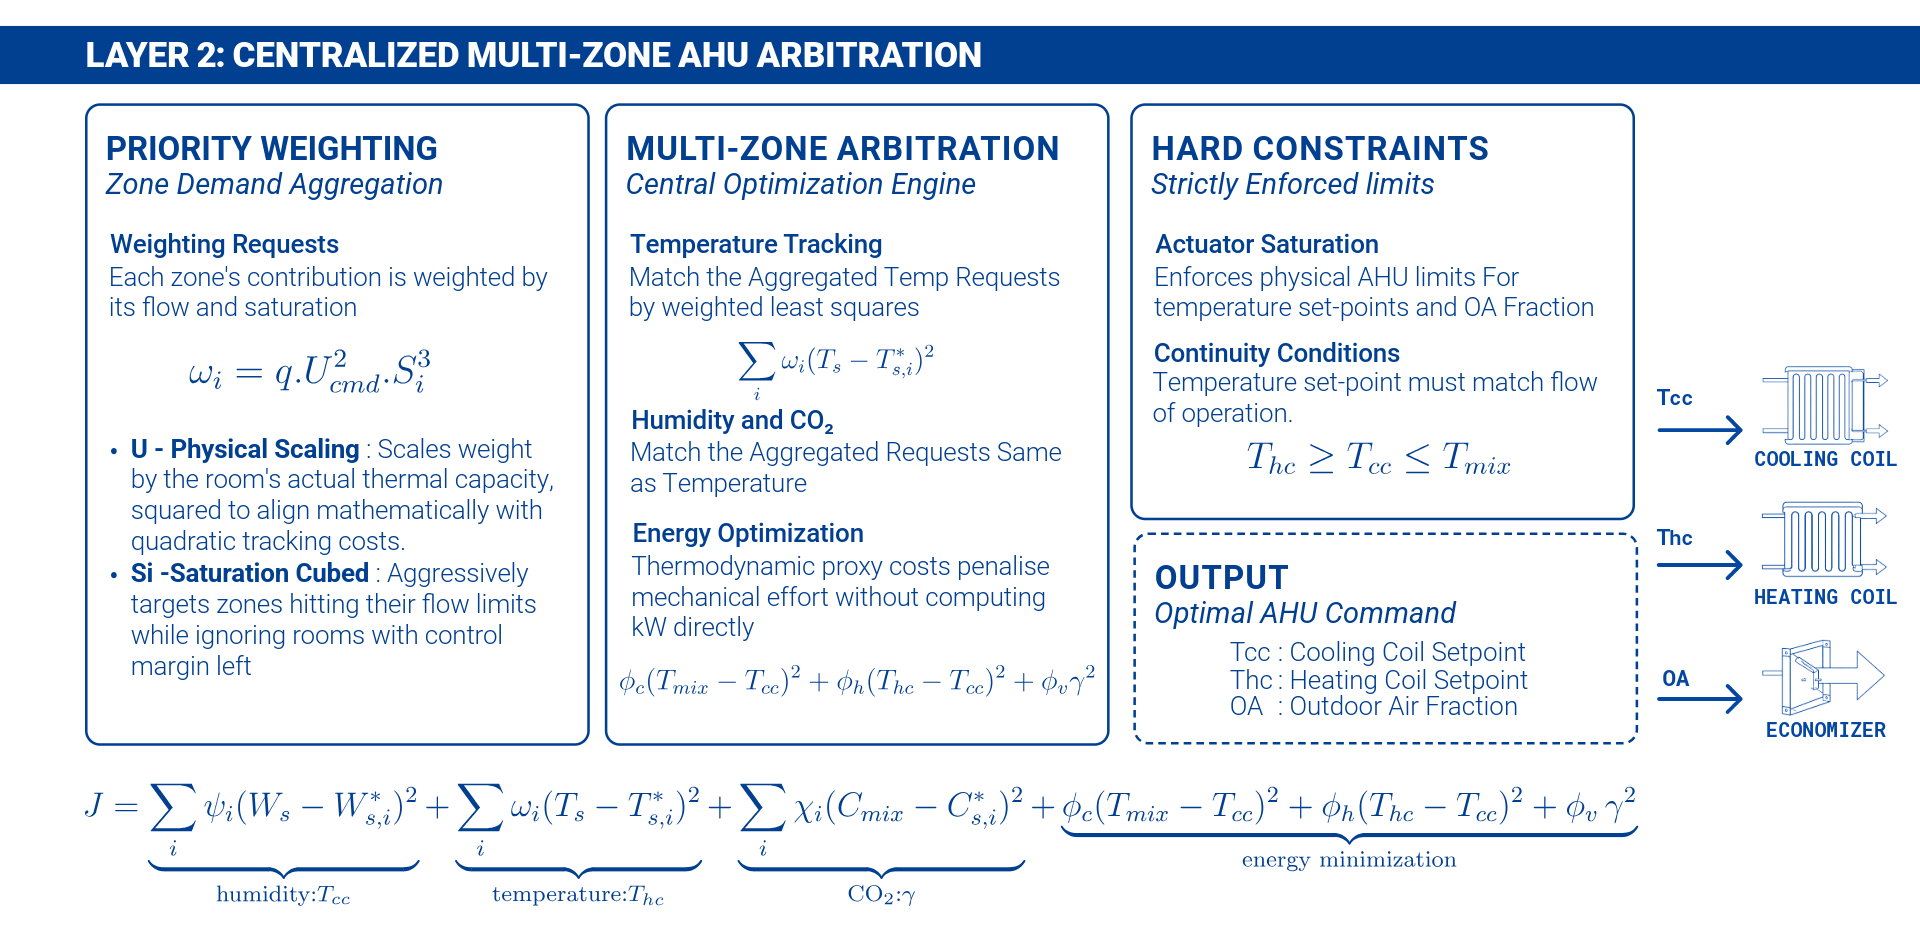
\includegraphics[width=1.0\textwidth]{images/fig_layer2_ahu_coordinator.png}
		\caption{Layer~2 - Central AHU Coordinator}
		\label{fig:layer2_ahu_coordinator}
	\end{figure}
	
	The Layer~2 controller acts as the central AHU coordinator, translating the individual zone requests generated by the Layer~1 controllers into a single physically consistent set of AHU operating commands. At each timestep, the coordinator receives one Ideal-Ask bundle from each zone. Where $T_{s,i}^{*}$, $W_{s,i}^{*}$, and $C_{s,i}^{*}$ are the requested supply air temperature, humidity ratio, and CO$_2$ concentration, respectively. The variables $u_{\mathrm{cmd},i}$ and $S_i$ describe the requested airflow and the degree to which the zone is approaching its available airflow capacity.
	\begin{equation}
		\mathcal{I}_i =
		\left\{
		T_{s,i}^{*},\;
		W_{s,i}^{*},\;
		C_{s,i}^{*},\;
		u_{\mathrm{cmd},i},\;
		S_i
		\right\}
	\end{equation}


	
	The coordinator determines three AHU level decision variables, 	where $T_{cc}$ is the cooling coil leaving air temperature, $T_{hc}$ is the heating coil leaving air temperature, and $\gamma$ is the outdoor air fraction. 
	\begin{equation}
		U_{\mathrm{AHU}} =
		\begin{bmatrix}
			T_{cc} & T_{hc} & \gamma
		\end{bmatrix}^{T}
	\end{equation}

	Where the humidity relationship is locally linearized around the current operating point. Cooling coil primarily determines the moisture content of the supply air, heating coil determines its temperature, and outdoor air fraction controlling CO$_2$ concentration.
	
	\subsubsection{Multi-Zone Weighting}
	
	Because a single AHU must satisfy competing requests from multiple zones, the coordinator assigns each zone a dynamic importance based on both its airflow demand and its proximity to the available flow limit. The temperature, humidity, and CO$_2$ tracking weights are defined as,

	\begin{equation}
\omega_i = q_T u_{\mathrm{cmd},i}^{2} S_i^{3}, \qquad \psi_i = q_W u_{\mathrm{cmd},i}^{2} S_i^{3}, \qquad \chi_i = q_C u_{\mathrm{cmd},i}^{2} S_i^{3}
	\end{equation}
	
	
	The squared commanded flow term, $u_{\mathrm{cmd},i}^{2}$, reflects the fact that a zone consuming a large portion of the AHU's available airflow represents a larger share of the available conditioning capacity and therefore has a greater influence on the required central operating point. Squaring the flow also prevents the weighting from increasing only linearly, providing stronger differentiation between low-flow and high-flow zones. The saturation term $S_i^{3}$ further increases the priority of zones approaching their airflow limit. The cubic dependence is intentionally stronger than the quadratic flow dependence. A zone operating near its flow ceiling receives a disproportionately larger weight because it has less remaining local control authority. 
	
	The coefficients $q_T$, $q_W$, and $q_C$ are normalization factors that account for the different numerical scales and units of temperature, humidity ratio, and CO$_2$ concentration. They establish comparable numerical contributions between the three controlled variables without changing the underlying priority mechanism.
	
	\subsubsection{Central Coordination Objective}
	
	The AHU operating point is selected by minimizing a combined tracking and energy objective,
	\begin{equation}
		\min_{T_{cc}, T_{hc}, \gamma}
		J
		=
		J_{\mathrm{track}}
		+
		J_{\mathrm{energy}}.
		\label{eq:coordinator_objective}
	\end{equation}
	
	\begin{equation}
		J_{\mathrm{track}}
		=
		\sum_i
		\psi_i
		\left(W_s-W_{s,i}^{*}\right)^2
		+
		\sum_i
		\omega_i
		\left(T_s-T_{s,i}^{*}\right)^2
		+
		\sum_i
		\chi_i
		\left(C_{\mathrm{mix}}-C_{s,i}^{*}\right)^2.
		\label{eq:J_track}
	\end{equation}
	
	Each term is associated with the AHU actuator that has the strongest physical influence over the corresponding variable. The humidity tracking term primarily determines the required cooling-coil condition through $T_{cc}$, the temperature tracking term determines the required heating-coil condition through $T_{hc}$, and the CO$_2$ tracking term determines the required outdoor-air fraction through $\gamma$. The squared tracking errors penalize large deviations more strongly than small deviations, causing the coordinator to prioritize substantial departures from the requested supply conditions while still considering the requirements of all zones.
	
	\begin{equation}
		J_{\mathrm{energy}} =
		\phi_c
		\left(T_{\mathrm{mix}}-T_{cc}\right)^2
		+
		\phi_h
		\left(T_{hc}-T_{cc}\right)^2
		+
		\phi_v\gamma^2.
		\label{eq:J_energy}	
	\end{equation}
	
	This term discourages unnecessary cooling, heating, and outdoor-air intake. The cooling and heating terms penalize excessive separation between the mixed-air condition and the coil operating temperatures, while the ventilation term discourages unnecessarily large outdoor-air fractions. These terms act as regularization of the central operating point, allowing the controller to select an energetically less demanding solution when multiple AHU operating points can provide similar zone-level performance. The coefficients $\phi_c$, $\phi_h$, and $\phi_v$ serve as normalization and relative-penalty factors for these three operating costs.
	
	\subsubsection{Hard Physical Constraints}
	
	The AHU optimization is subject to hard physical constraints that define the feasible operating region of the cooling coil, heating coil, and outdoor-air damper. These constraints are imposed directly on the optimization and therefore cannot be violated in favour of improved tracking or reduced energy use. The resulting feasible set preserves the physical operating sequence of the AHU while preventing infeasible actuator commands.
	
	\begin{table}[h!]
		\centering
		\caption{Hard physical constraints imposed on the AHU coordinator.}
		\label{tab:ahu_hard_constraints}
		\renewcommand{\arraystretch}{1.25}
		\begin{tabular}{p{0.25\textwidth} p{0.27\textwidth} p{0.38\textwidth}}
			\toprule
			\textbf{Constraint} & \textbf{Mathematical limit} & \textbf{Physical purpose} \\
			\midrule
			Cooling-coil temperature
			&
			$T_{c,\min} \leq T_{cc} \leq T_{\mathrm{mix}}$
			&
			Restricts the cooling-coil leaving-air temperature to its admissible range while ensuring that the coil operates in the cooling direction relative to the mixed air stream.
			\\
			
			Heating-coil temperature
			&
			$T_{cc} \leq T_{hc} \leq T_{c,\max}$
			&
			Constrains the downstream heating coil to operate at or above the cooling coil leaving temperature while remaining within the allowable upper temperature limit.
			\\
			
			Outdoor-air fraction
			&
			$\gamma_{\min} \leq \gamma \leq 1$
			&
			Ensures the required minimum outdoor-air provision while allowing operation up to full outdoor-air conditions.
			\\
			\bottomrule
		\end{tabular}
	\end{table}
	
	These constraints directly represent the physical sequence of the AHU. The cooling coil first reduces the mixed-air temperature, giving $T_{cc} \leq T_{\mathrm{mix}}$, after which the heating coil can only maintain or increase the air temperature, giving $T_{hc} \geq T_{cc}$. The upper bound on $T_{hc}$ prevents excessive supply air temperatures, while the lower bound on $T_{cc}$ prevents operation below the specified cooling coil limit. The outdoor air constraint independently maintains the required minimum ventilation level.

	\newpage
	
	
	\section{Implementation and Experimental Setup}
	
	\subsection{Simulation Environment}
	
	\subsubsection{EnergyPlus Building Model}
	
	Validation of the full multi-zone control architecture was conducted using EnergyPlus Version 25.1.0, the U.S. Department of Energy's open-source building energy simulation engine. The standard \texttt{5ZoneAutoDXVAV} reference model was selected as the simulation testbed, and its building geometry is shown in Figure~\ref{fig:sim_model}. This model represents a single-storey commercial building partitioned into five thermally distinct zones (SPACE1-1 through SPACE5-1), each served by an individual Variable Air Volume (VAV) damper box. All five zones share a single central Air Handling Unit comprising a direct-expansion (DX) cooling coil, a gas heating coil, an economizer damper, and a supply fan, making it a physically realistic representation of the shared-resource multi-zone problem this project addresses.
	
	\begin{figure}[ht]
		\centering
		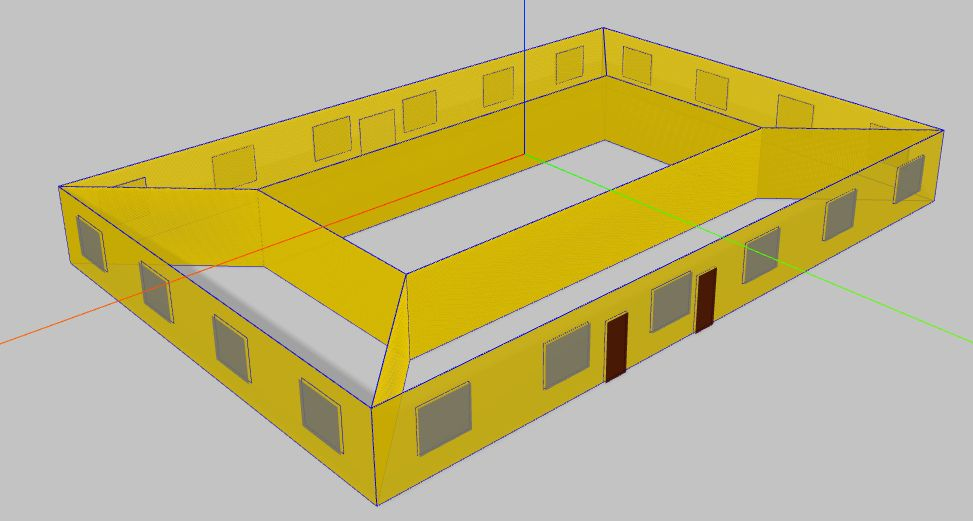
\includegraphics[width=0.75\linewidth]{images/fig_sim_model.png}
		\caption{Building geometry of the \texttt{5ZoneAutoDXVAV} EnergyPlus reference model.}
		\label{fig:sim_model}
	\end{figure}
	
	All simulations were conducted using the Sri Lankan weather dataset (Colombo Katunayake) to reflect the tropical climate context motivating this work. Table~\ref{tab:ep_config} summarises the key simulation configuration parameters.
	
	\begin{table}[h]
		\centering
		\caption{EnergyPlus Simulation Configuration}
		\label{tab:ep_config}
		\begin{tabular}{ll}
			\toprule
			\textbf{Parameter} & \textbf{Value} \\
			\midrule
			EnergyPlus Version      & 25.1.0-68a4a7c774 \\
			Building Model          & 5ZoneAutoDXVAV (5 zones, single AHU) \\
			Weather File            & Colombo Katunayake, Sri Lanka \\
			AHU Configuration       & DX cooling coil, gas heating coil, economizer, supply fan \\
			Zone Actuator           & VAV damper per zone \\
			Timestep                & 6 steps per hour (10-minute intervals) \\
			\bottomrule
		\end{tabular}
	\end{table}

	\subsubsection{Python Plugin Architecture}
	
	The custom control logic is embedded into the simulation using the EnergyPlus Python Plugin interface. The plugin intercepts the simulation at two critical callback hooks per timestep,
	
	\begin{itemize}
		\item \texttt{on\_begin\_timestep\_before\_predictor} - reads sensor handles, runs the EKF and zone MPC for each zone, and issues VAV damper commands.
		\item \texttt{on\_inside\_hvac\_system\_iteration\_loop} - reads AHU system states, runs the AHU Coordinator QP, and writes cooling coil, heating coil, outdoor-air fraction, and humidifier setpoints to their respective actuator handles.
	\end{itemize}
	
	This dual callback structure mirrors the physical separation between zone-level and supervisory control. Zone controllers act before the HVAC predictor, and the AHU coordinator acts inside the HVAC iteration loop. The plugin dynamically discovers the active thermal zones at initialisation and instantiates one \texttt{ZoneController} object per zone and a single shared \texttt{AHUCoordinator}. All simulation state is logged to a timestep resolution CSV file, which was subsequently used for result analysis and validation. The full implementation is available in the open repository \texttt{https://github.com/janithcyapa/DHCA-Framework}.
	
	\subsubsection{Supplementary Occupancy Dataset}
	
	To emulate realistic and chaotic occupancy disturbances across the five zones, the ROBOD dataset (Room-level Occupancy and Building Operation Dataset) (~\cite{robod2022}) was used as the supplementary data source. Per-zone occupancy schedules were drawn from this dataset and injected into the simulation at each timestep, alongside stochastic plug load and lighting profiles. Temperature setpoints were varied using randomised block schedules seeded per zone, holding a randomly drawn setpoint between 20°C and 25°C for eight-hour blocks, to test controller robustness under non-stationary reference tracking. The ROBOD dataset is publicly available at \url{https://doi.org/10.6084/m9.figshare.19234530}.
	
	\newpage
	
	\subsection{Hardware Implementation}
	
	\subsubsection{Controller Hardware}
	
	The physical hardware of the decentralised zone controller was built around the ESP32 microcontroller, programmed using the ESP-IDF (Espressif IoT Development Framework) in C++. The ESP32 was selected for its dual-core processing capability, integrated Wi-Fi, and the mature real time operating system support provided by ESP-IDF, which allows sensor polling, control computation, and wireless communication to run as concurrent FreeRTOS tasks.
	
	A custom Printed Circuit Board (PCB) was designed and fabricated to serve as a unified plug-and-play interface for the ESP32. The PCB integrates all peripheral connections onto a single board, eliminating loose wiring and reducing electrical noise. The PCB layout is  shown in Figure~\ref{fig:pcb_design} and  the assembled controller device is  shown in Figure~\ref{fig:controller_device}. Table~\ref{tab:pcb_peripherals} lists the key peripheral interfaces routed on the PCB.
	
	\begin{figure}[H]
		\centering
		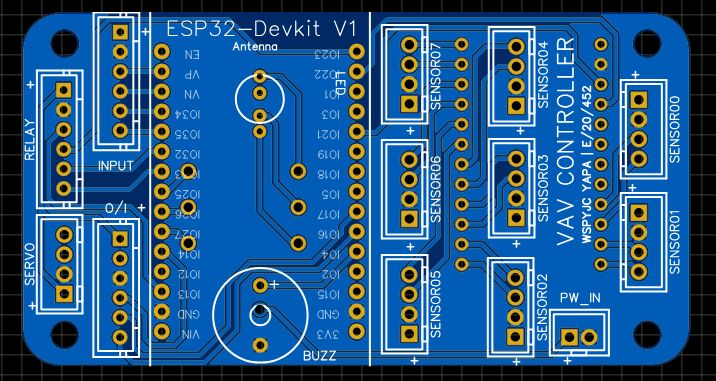
\includegraphics[width=0.75\linewidth]{images/fig_pcb_design.png}
		\caption{PCB layout of the custom ESP32 shield.}
		\label{fig:pcb_design}
	\end{figure}
	
	\begin{table}[h]
		\centering
		\caption{Custom PCB Peripheral Interface Summary}
		\label{tab:pcb_peripherals}
		\begin{tabular}{lll}
			\toprule
			\textbf{Peripheral} & \textbf{Interface} & \textbf{GPIO} \\
			\midrule
			I2C Multiplexer (PCA9548A) & I2C          & SDA: GPIO 21, SCL: GPIO 22 \\
			Cooling coil relay         & Digital output & GPIO 13 \\
			Heating coil relay         & Digital output & GPIO 33 \\
			Humidifier relay           & Digital output & GPIO 32 \\
			Economizer damper servo    & PWM            & GPIO 19 \\
			Main blower servo          & PWM            & GPIO 18 \\
			\bottomrule
		\end{tabular}
	\end{table}
	
	\begin{figure}[H]
		\centering
		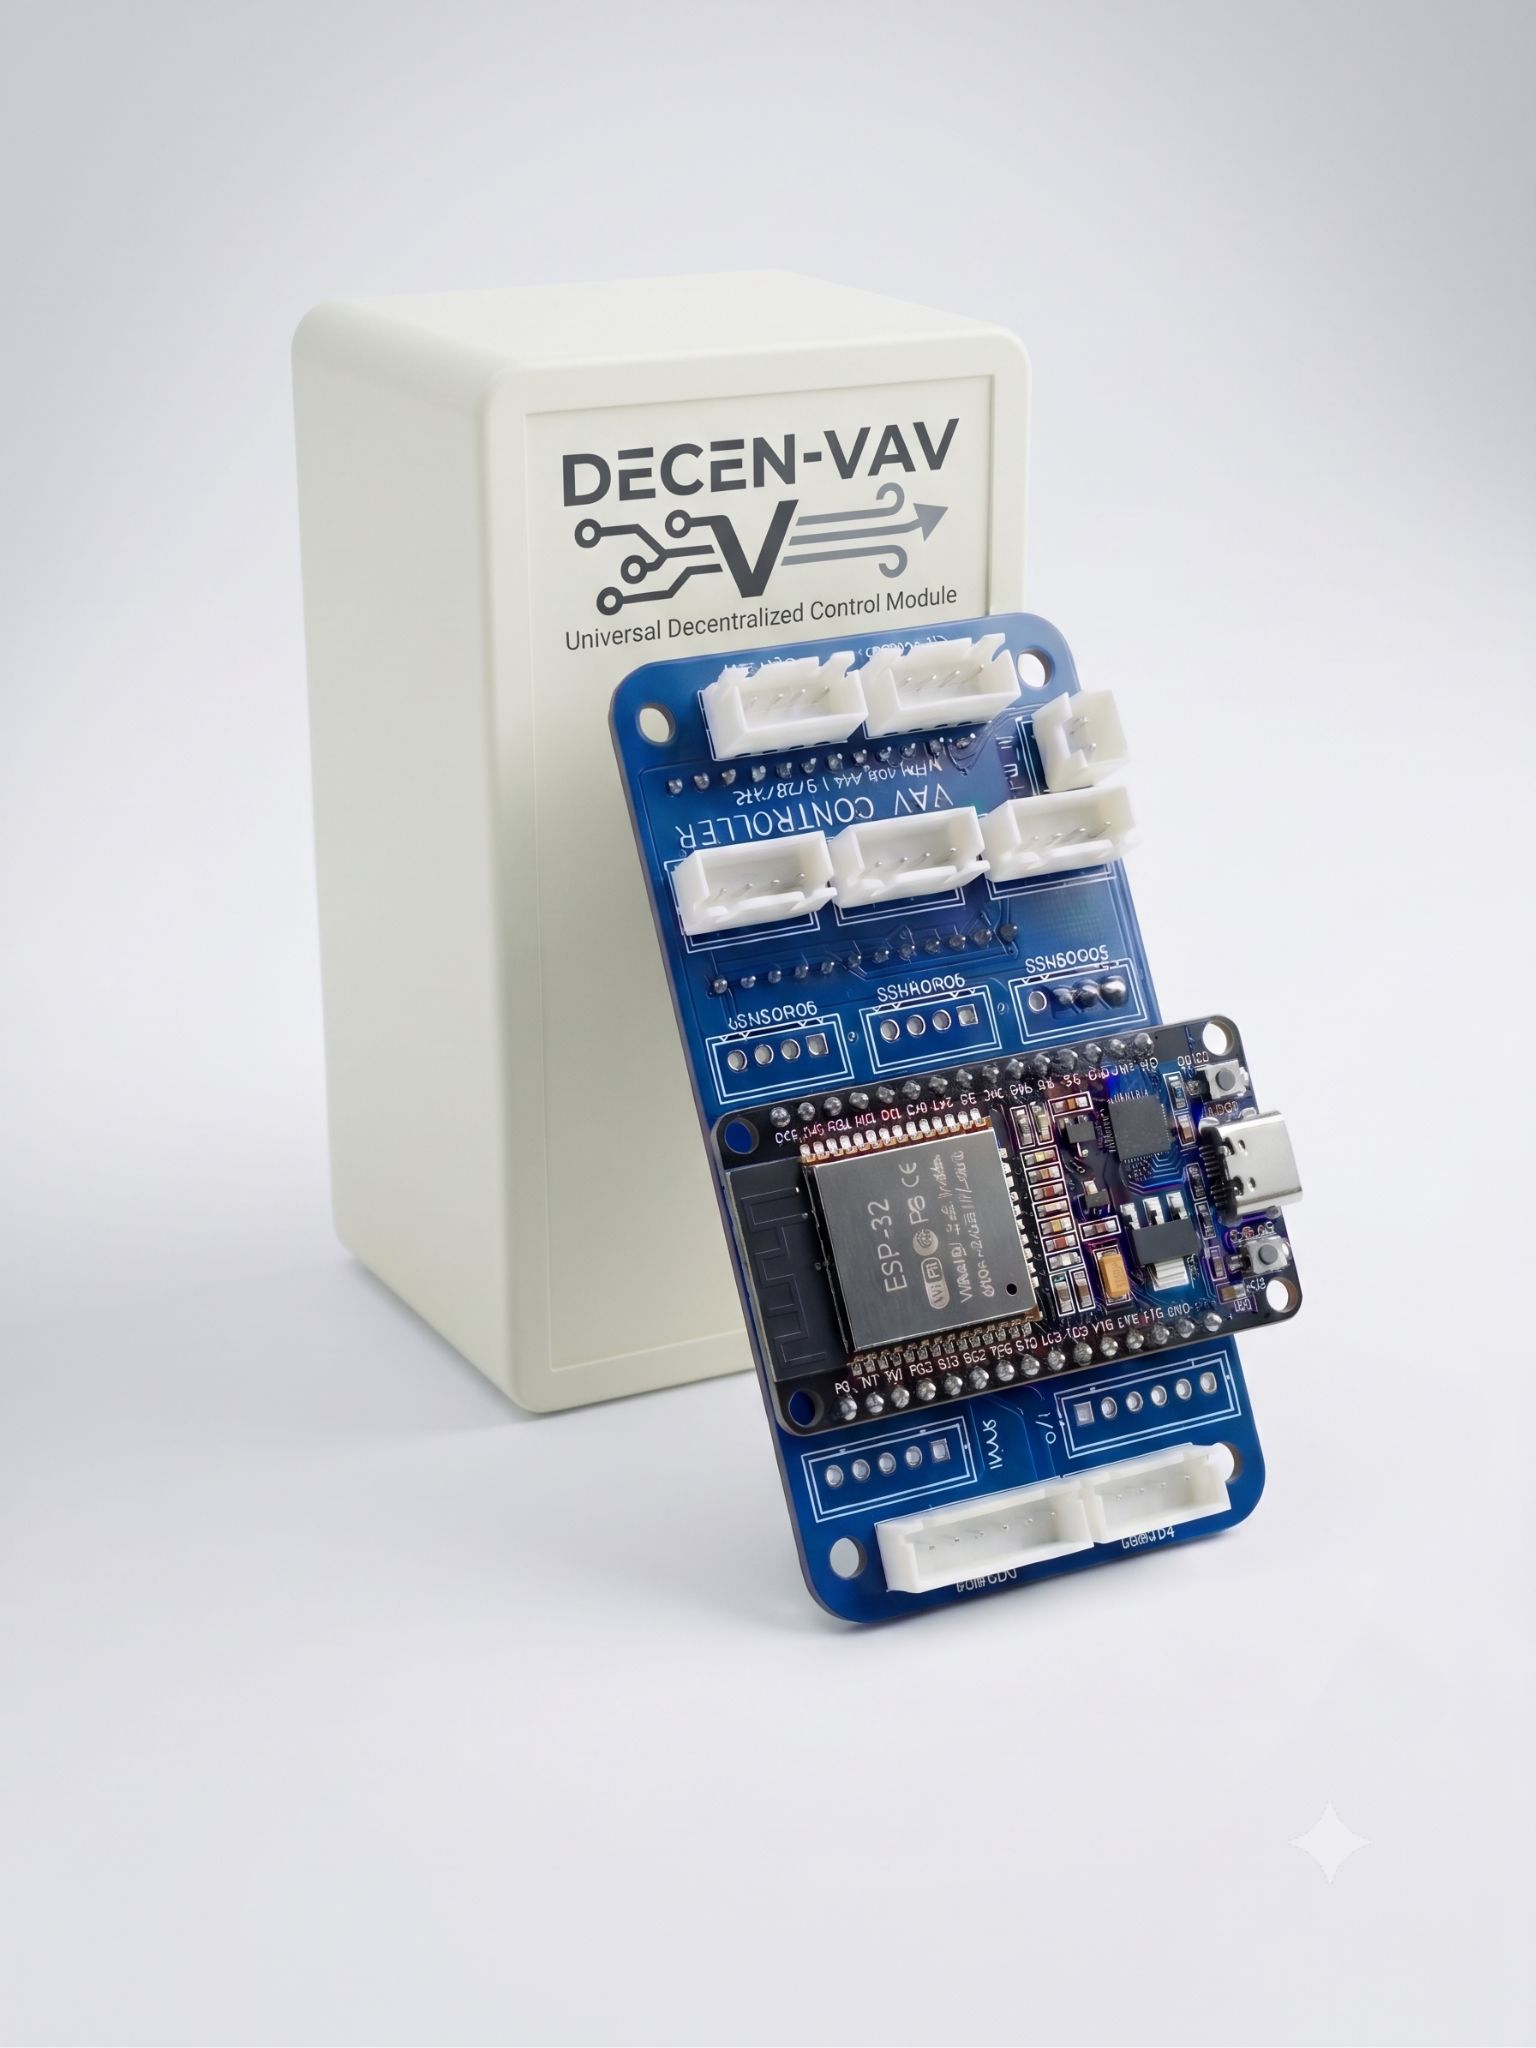
\includegraphics[width=0.65\linewidth]{images/fig_zone_controller_hardwear.png}
		\caption{Assembled DECEN-VAV zone controller module in its enclosure.}
		\label{fig:controller_device}
	\end{figure}
	

	
	\subsubsection{Sensing Suite}
	
	Each zone node was equipped with two digital environmental sensors interfaced over I2C.
	
	\begin{itemize}
		\item \textbf{BME280} -  measures dry-bulb temperature, relative humidity, and barometric pressure. This sensor provides the $T_{in}$ and $W_{in}$ measurements consumed by the EKF at each timestep.
		\item \textbf{ENS160} - measures equivalent CO$_2$ (eCO$_2$) concentration. This provides the $C_{in}$ measurement for the EKF's CO$_2$ state update.
	\end{itemize}
	
	The I2C multiplexer architecture allows multiple sensors with identical I2C addresses to coexist on the same bus, enabling  distribution of sensing nodes within a single zone without  conflicts. Table~\ref{tab:sensors} summarises the key sensor specifications.
	
	\begin{table}[h]
		\centering
		\caption{Environmental Sensing  Specifications}
		\label{tab:sensors}
		\begin{tabular}{lllll}
			\toprule
			\textbf{Sensor} & \textbf{Measurement} & \textbf{EKF State} & \textbf{Interface} & \textbf{I2C Address} \\
			\midrule
			BME280 & Temperature ($^\circ$C)      & $T_{in}$   & I2C & \texttt{0x76} \\
			BME280 & Relative Humidity (\% RH)    & $W_{in}$   & I2C & \texttt{0x76} \\
			ENS160 & eCO$_2$ (ppm)                & $C_{in}$   & I2C & \texttt{0x53} \\
			\bottomrule
		\end{tabular}
	\end{table}
	
	\subsubsection{Air Flow Calibration}
	
	Because the physical testbench fan and OA damper does not directly report volumetric flow, flow rates were calibrated using an anemometer measurements  across the fan command and mixer damper operating range. Table~\ref{tab:flow_calibration} summarises the measured total system flow at key operating points, and Table~\ref{tab:mixer_flow} summarises the economizer mixer contribution.
	
	\begin{table}[h]
		\centering
		\caption{Total Actual System Flow at  Main Duct (m$^3$/h)}
		\label{tab:flow_calibration}
		\begin{tabular}{ccc}
			\toprule
			\textbf{Fan Command} & \textbf{Mixer 0\%} & \textbf{Mixer 100\%} \\
			\midrule
			40\% & 75.3 & 88.9 \\
			50\% & 164.2 & 184.7 \\
			60\% & 270.3 & 301.0 \\
			70\% & 301.0 & 331.8 \\
			80\% & 311.3 & 338.7 \\
			\bottomrule
		\end{tabular}
	\end{table}
	
	\begin{table}[h]
		\centering
		\caption{Economizer Mixer Contribution Flow (m$^3$/h)}
		\label{tab:mixer_flow}
		\begin{tabular}{ccccc}
			\toprule
			\textbf{Fan Command} & \textbf{M=25\%} & \textbf{M=50\%} & \textbf{M=75\%} & \textbf{M=100\%} \\
			\midrule
			50\% & 7.0 & 54.7 & 82.6 & 72.0 \\
			60\% & 11.2 & 69.1 & 127.9 & 136.8 \\
			70\% & 12.6 & 74.9 & 138.5 & 151.2 \\
			\bottomrule
		\end{tabular}
	\end{table}
	
	From these measurements, two flow models were fitted. The total system flow $F_{act}$ (m$^3$/s) and economizer mixer flow $F_{mix}$ (m$^3$/s) are described by the following  functions, where $C$ is the fan command percentage and $M$ is the mixer damper opening percentage.
	
	\begin{equation}
		F_{act} = \frac{0.0884 + 0.000076M}{1 + e^{-0.16(C - 49 + 0.01M)}}
	\end{equation}
	
	\begin{equation}
		F_{mix} = \frac{0.0431}{\left(1 + e^{-0.18(C-52)}\right)\left(1 + e^{-0.08(M-50)}\right)}
	\end{equation}
	
	Because $F_{mix}$ depends on both $C$ and $M$, and $F_{act}$ depends weakly on $M$, the inversion from target flows to actuator commands is solved numerically.
	
	\newpage
	
	\subsection{Telemetry and Monitoring Interface}
	
	A real-time web dashboard was developed to monitor the experimental testbench and support manual override during data collection. The firmware, implemented in C++ under ESP-IDF, configures the ESP32 as a standalone Wi-Fi Access Point. The dashboard application, built with React and TypeScript and compiled to a gzip-compressed static bundle served directly from the ESP32's flash memory, connects to the device via WebSocket at \texttt{ws://192.168.4.1/ws}.
	
	The telemetry architecture uses a structured JSON payload published by the ESP32 at high frequency, containing live readings from all sensors, current actuator positions, and EKF state estimates. The dashboard provides bidirectional communication: it renders live readings of temperature, humidity, CO$_2$  and pressure at each point and transmits actuator command objects back to the ESP32, allowing the operator to switch between autonomous control mode and manual override without interrupting the sensor logging pipeline. The dashboard interface is shown in Figure~\ref{fig:dashboard}. The full hardware firmware and dashboard source are available at the repository \texttt{janithcyapa/MechLabs\_AHU}.
	
	\begin{figure}[ht]
		\centering
		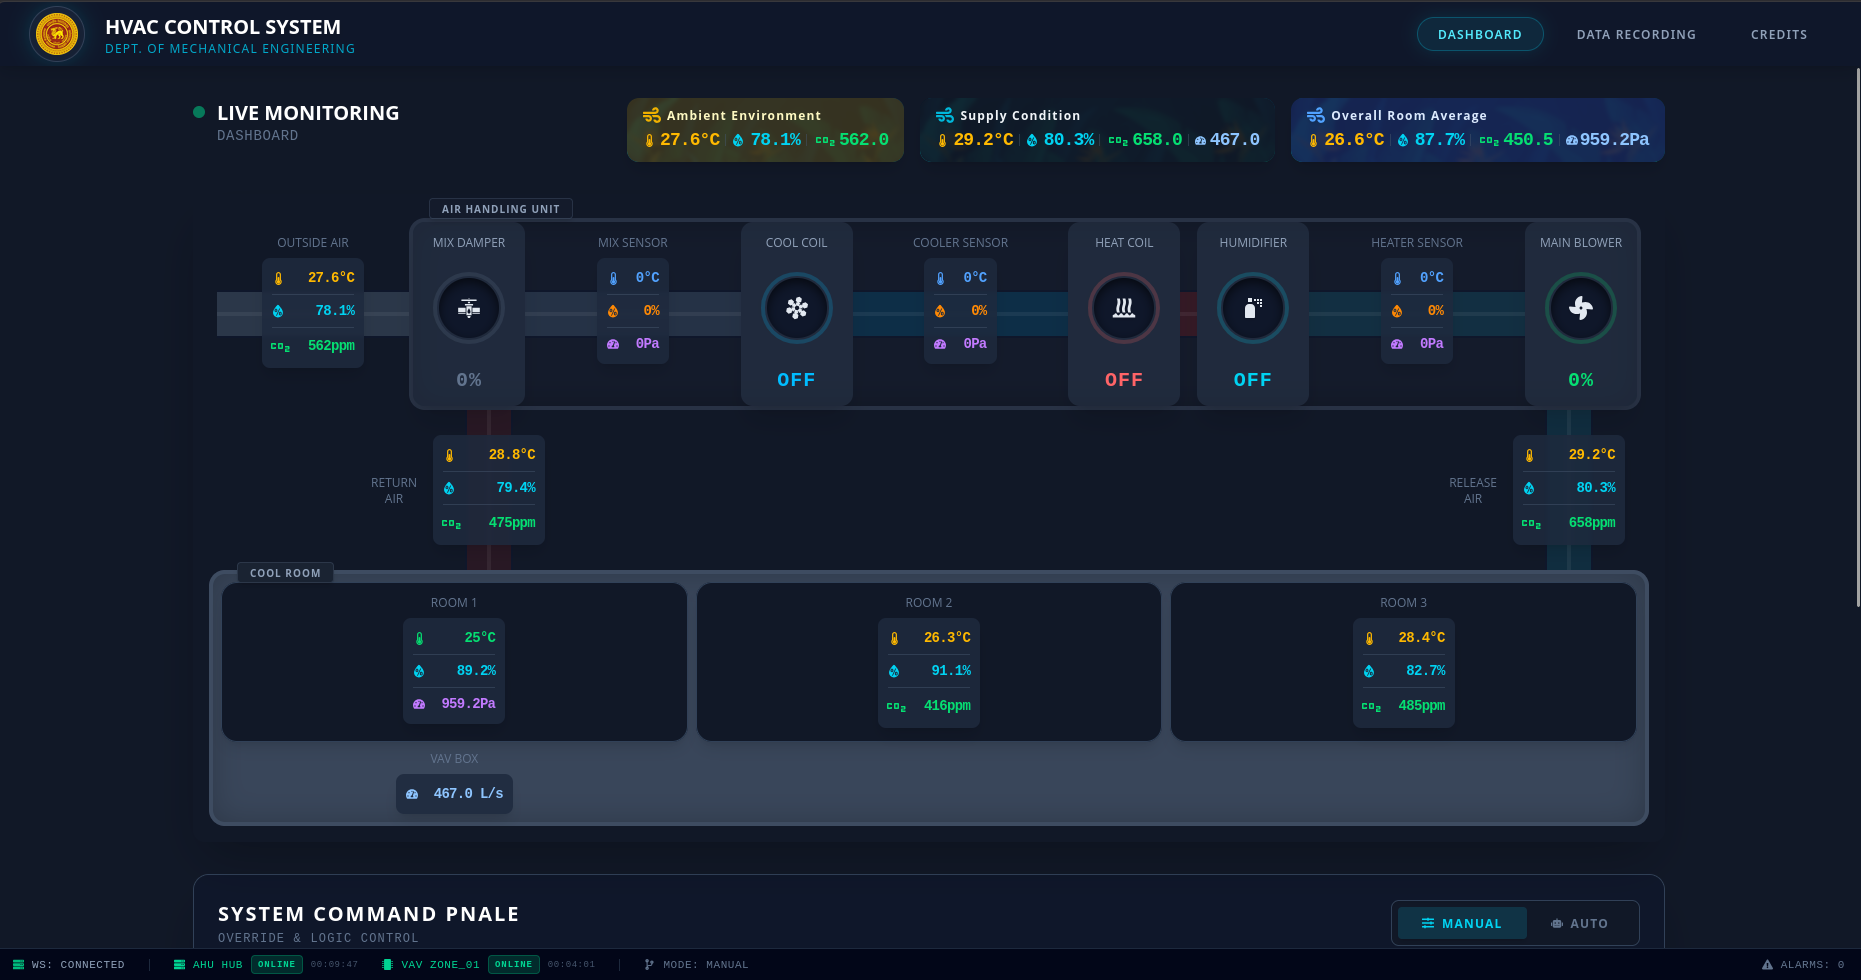
\includegraphics[width=1.0\linewidth]{images/fig_dashboard.png}
		\caption{Real-time web dashboard and DAQ}
		\label{fig:dashboard}
	\end{figure}
	\newpage
	
	\subsection{Single-Zone Experimental Testbench}
	
	The experimental validation was conducted using an existing single-zone cool-room HVAC testbench. The original system is a mostly analog air conditioning plant comprising an economiser, cooling coil, heating coil, humidifier, and supply fan serving a single conditioned room. Rather than replacing or redesigning the existing HVAC system, the testbench was used as the physical plant and digitally retrofitted to provide the sensing and actuation required by the proposed controller digitally.
	
	A secondary digital control layer was added to the existing system, incorporating digital temperature, humidity, and CO$_2$ sensing together with the required actuators at economizer and fan. This allowed the proposed zone level controller to operate the physical plant while preserving its original HVAC components and operating sequence. Since the testbench serves only a single room and does not contain a dedicated VAV damper, the supply fan speed is used as the equivalent airflow control actuator, allowing the zone controller to regulate the airflow supplied to the room. The resulting setup provides a practical hardware environment in which the controller can be evaluated under sensor noise, communication delays, actuator limitations, and unmodelled dynamics that are not fully represented in simulation. Figure~\ref{fig:experimental_setup} shows the instrumented testbench, digital sensor nodes, actuator interfaces, and the installed control and monitoring hardware.
	
	\begin{figure}[ht]
		\centering
		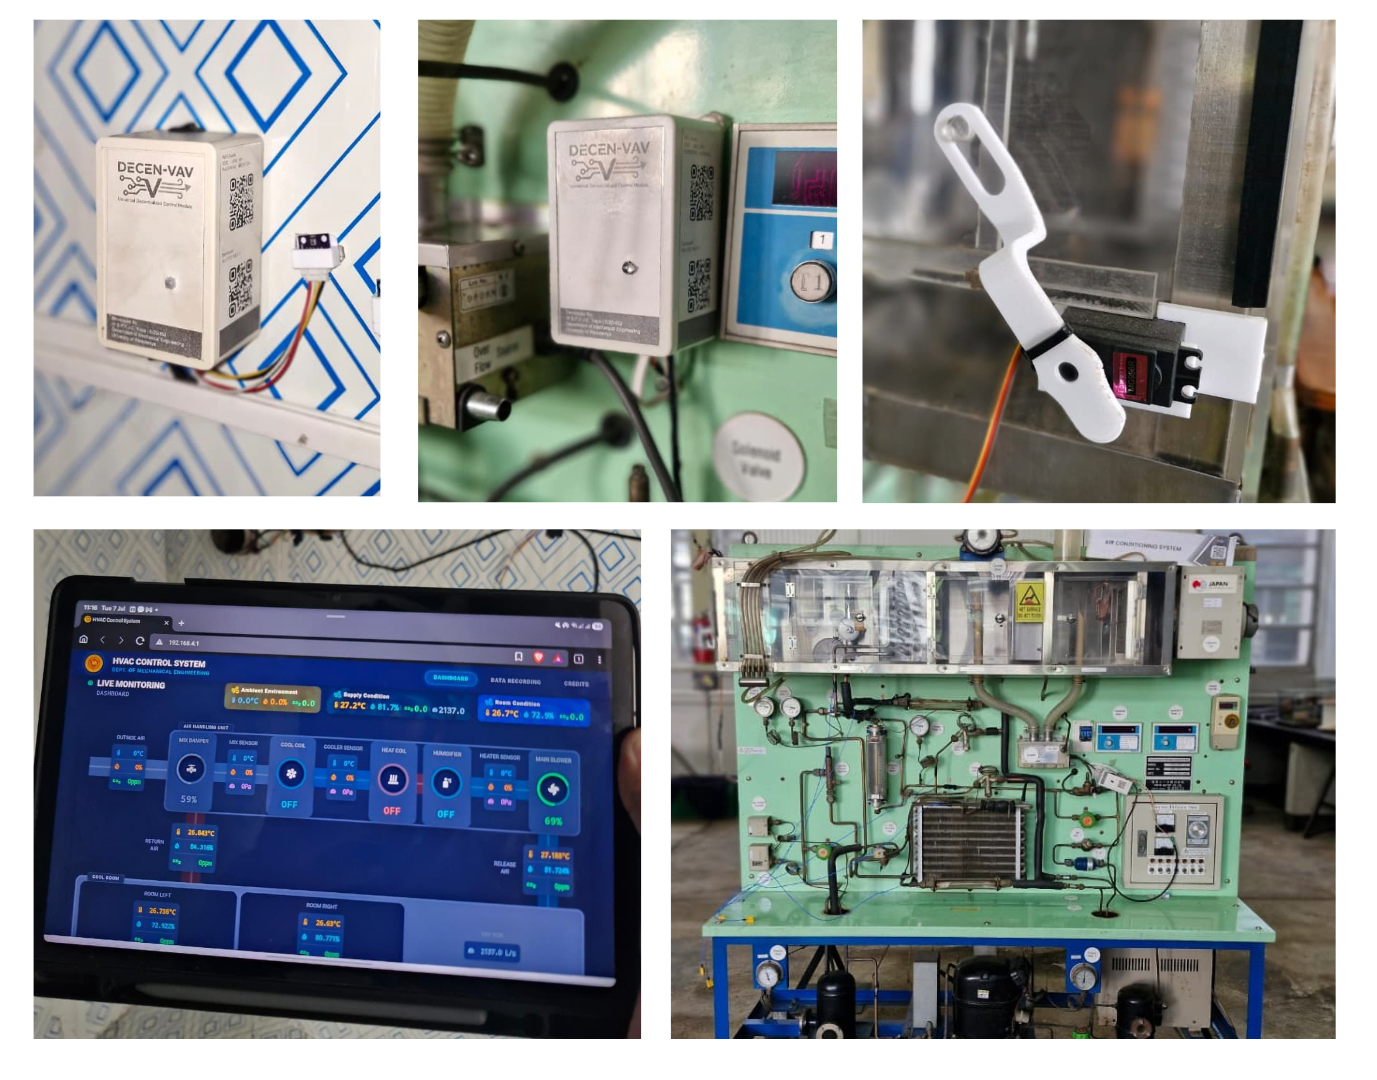
\includegraphics[width=\linewidth]{images/fig_experimental_setup.png}
		\caption{Single-zone experimental testbench with the digitally retrofitted sensing and control layer.}
		\label{fig:experimental_setup}
	\end{figure}
	
	\newpage
	
	\section{Results}
	
	% ------------------------------------------------------------
	\subsection{Simulation Validation within EnergyPlus}
	\label{sec:results_sim}
	% ------------------------------------------------------------
	
	
	% ------------------------------------------------------------
	\subsubsection{EKF State Tracking and Normalised Innovation Squared Health}
	\label{sec:results_ekf}
	% ------------------------------------------------------------
	
	Before evaluating closed-loop comfort performance it is necessary to
	confirm that the Extended Kalman Filter is producing reliable state and
	disturbance estimates, since every control decision depends on
	the filter output.  Figure~\ref{fig:ekf_space3} shows the EKF diagnostics
	for SPACE3-1, selected as a representative zone because it experiences the
	most variable occupancy schedule in the dataset.
	
	\begin{figure}[htbp]
		\centering
		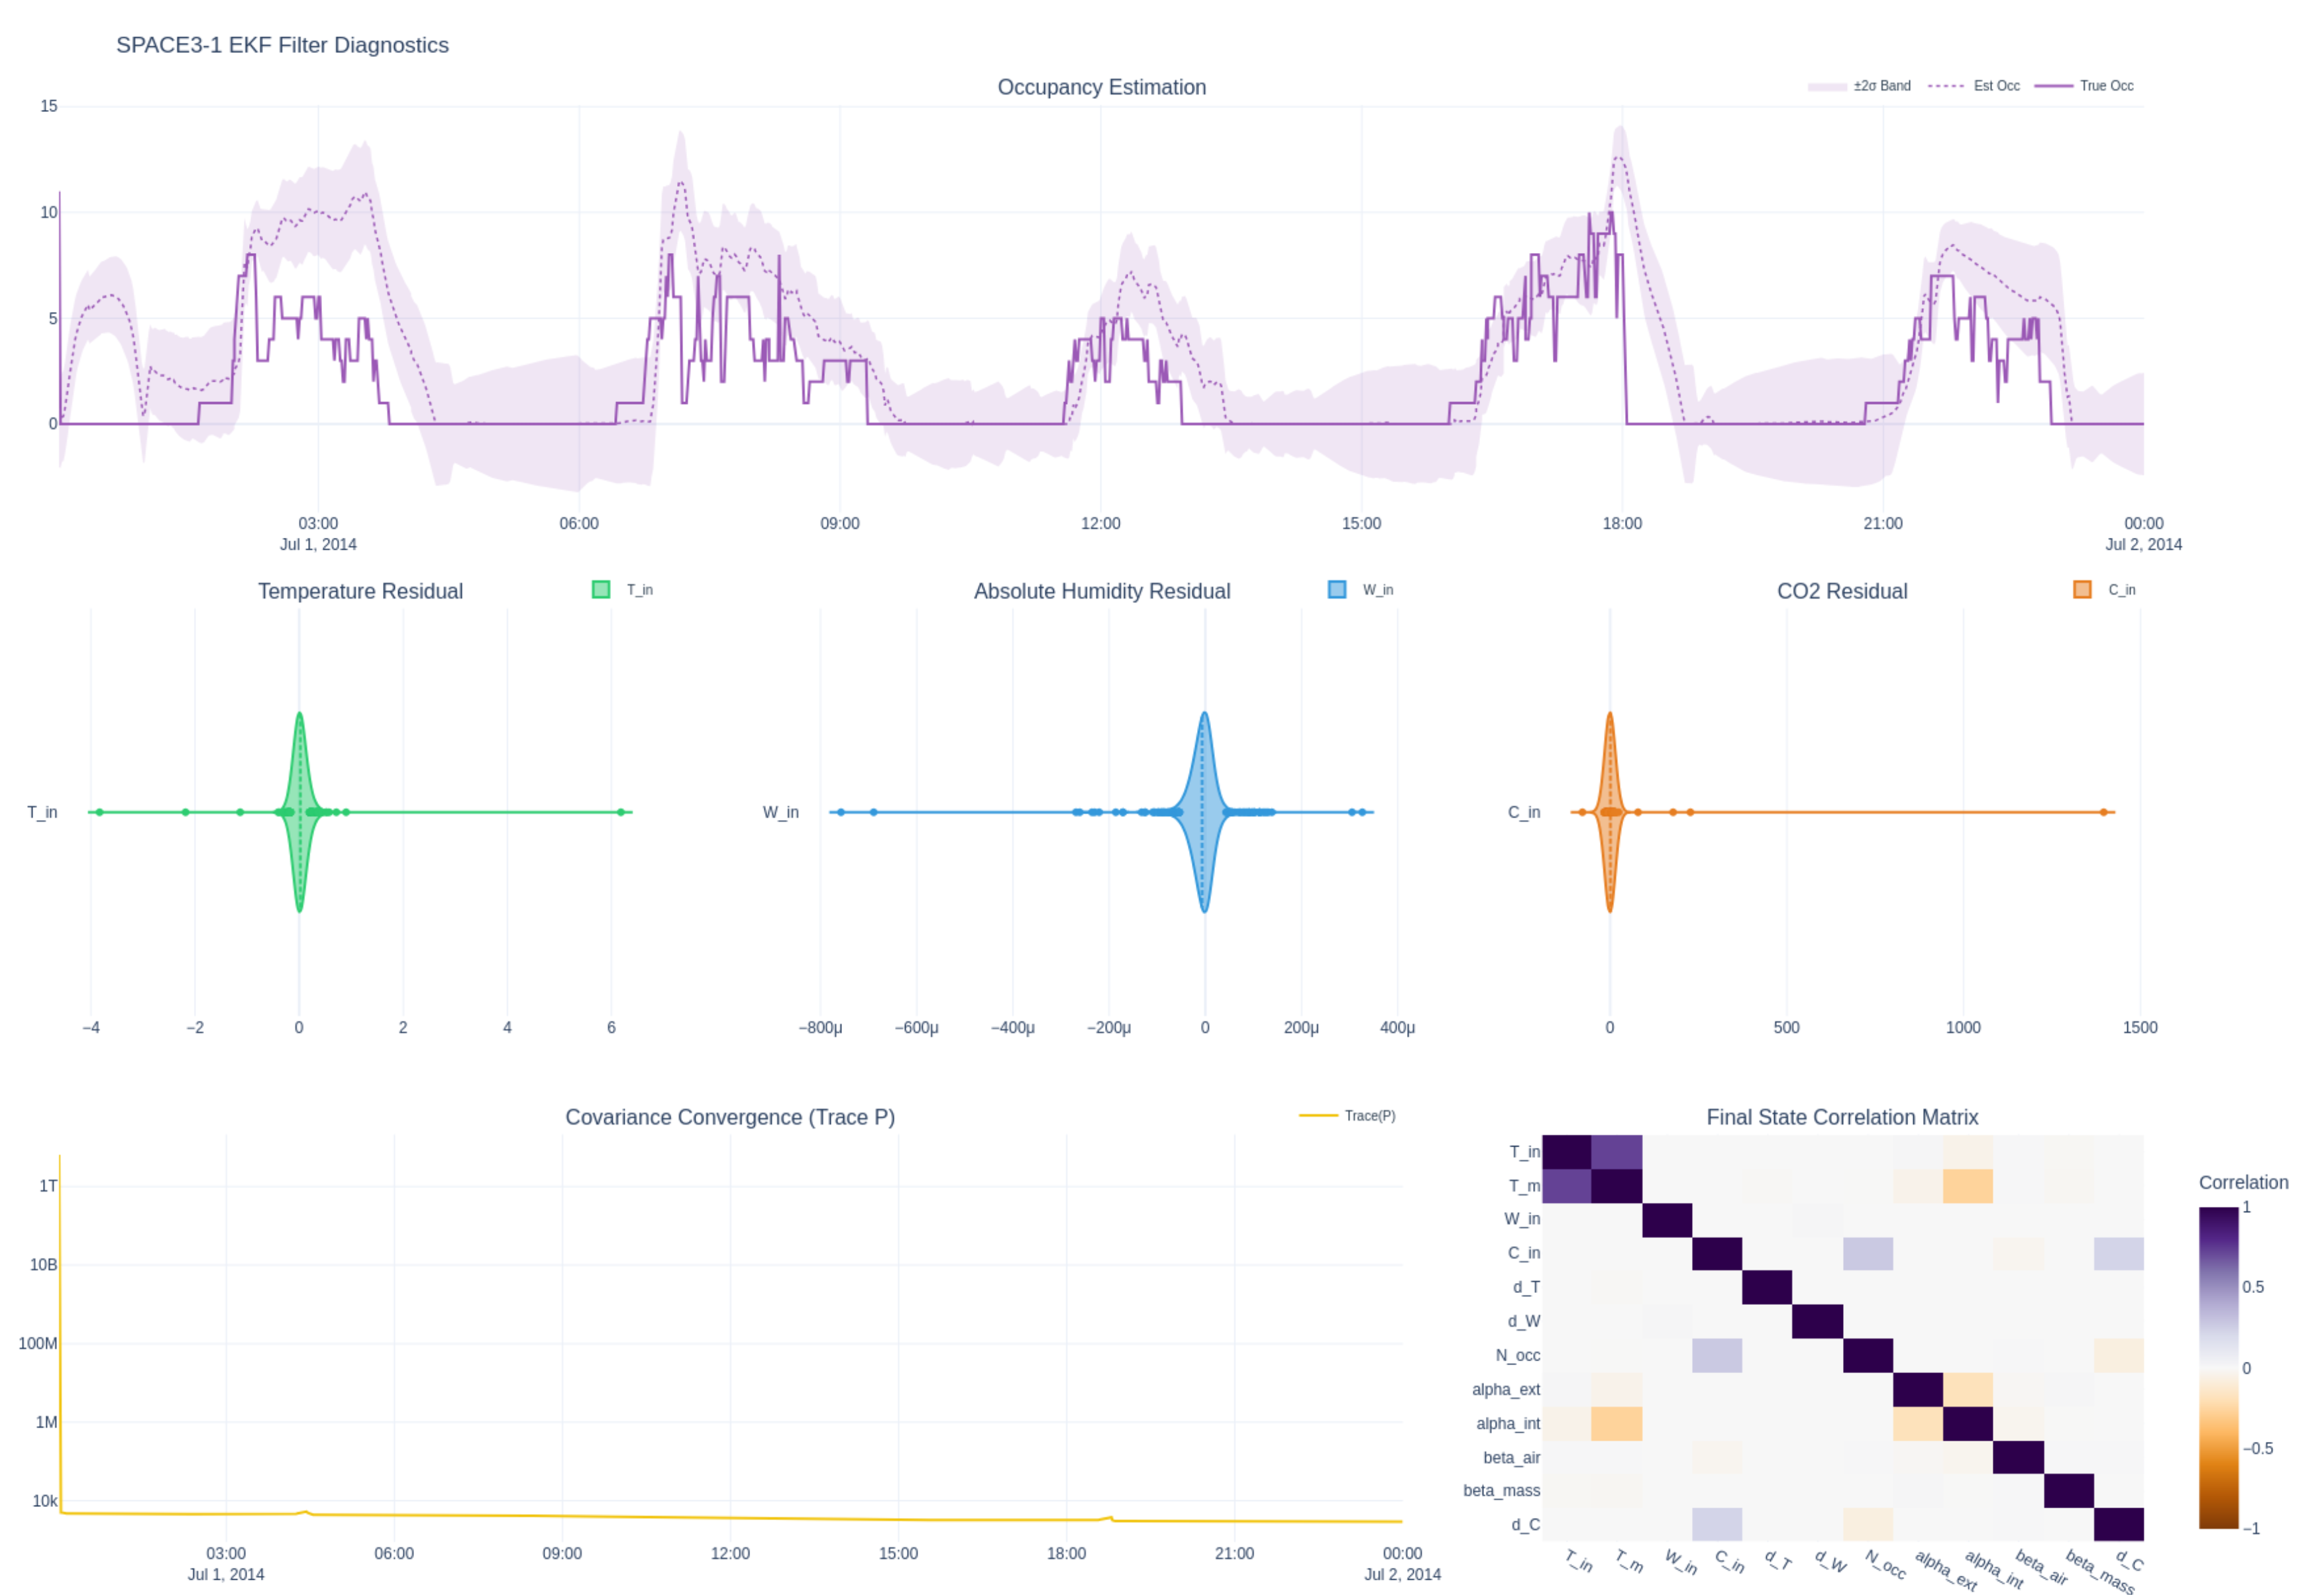
\includegraphics[width=1.0\linewidth]{results/fig_ekf_space3.png}
		\caption{EKF diagnostics for SPACE3-1}
		\label{fig:ekf_space3}
	\end{figure}
	
	Four features confirm filter health.  First, the occupancy estimate
	tracks the stochastic true count within the $\pm 2\sigma$ band throughout
	both occupied and unoccupied periods, demonstrating that the slowly decaying
	latent occupancy state absorbs the irregular respiration and moisture loads
	without requiring a direct occupancy sensor.  Second, the innovation
	distributions are centred near zero and confined to a narrow band relative
	to sensor noise, indicating that the predicted and measured values are
	statistically consistent.  The covariance trace $\mathrm{Tr}(P)$
	drops by more than six orders of magnitude within the first two hours of
	simulation, after which it stabilises, indicating that the filter has
	converged and is no longer dependent on its initialisation.  The
	final-state correlation matrix shows that the physical-parameter states
	$\alpha_{ext}$, $\alpha_{int}$, $\beta_{air}$, $\beta_{mass}$ remain largely
	decorrelated from the disturbance states, confirming that the two
	estimation tasks do not interfere with each other.

	\subsubsection{Multi-Zone Temperature Regulation with Independent Setpoints}
	
	The primary objective of the architecture is that each zone controller
	operates individually and that zones with different temperature setpoints can
	coexist under a shared AHU without any zone overriding another.
	Figure~\ref{fig:allzone_temp} demonstrates this across the full 31-day
	simulation.  Each of the five zones follows its own independently randomised
	temperature setpoint schedule, and in each case the zone temperature remains within the
	$\pm 1\,^\circ$C deadband for the majority of occupied hours. The optimizer status strip at
	the bottom shows for timesteps both stages were solved under the given constraints. 
	
	\begin{figure}[htbp]
		\centering
		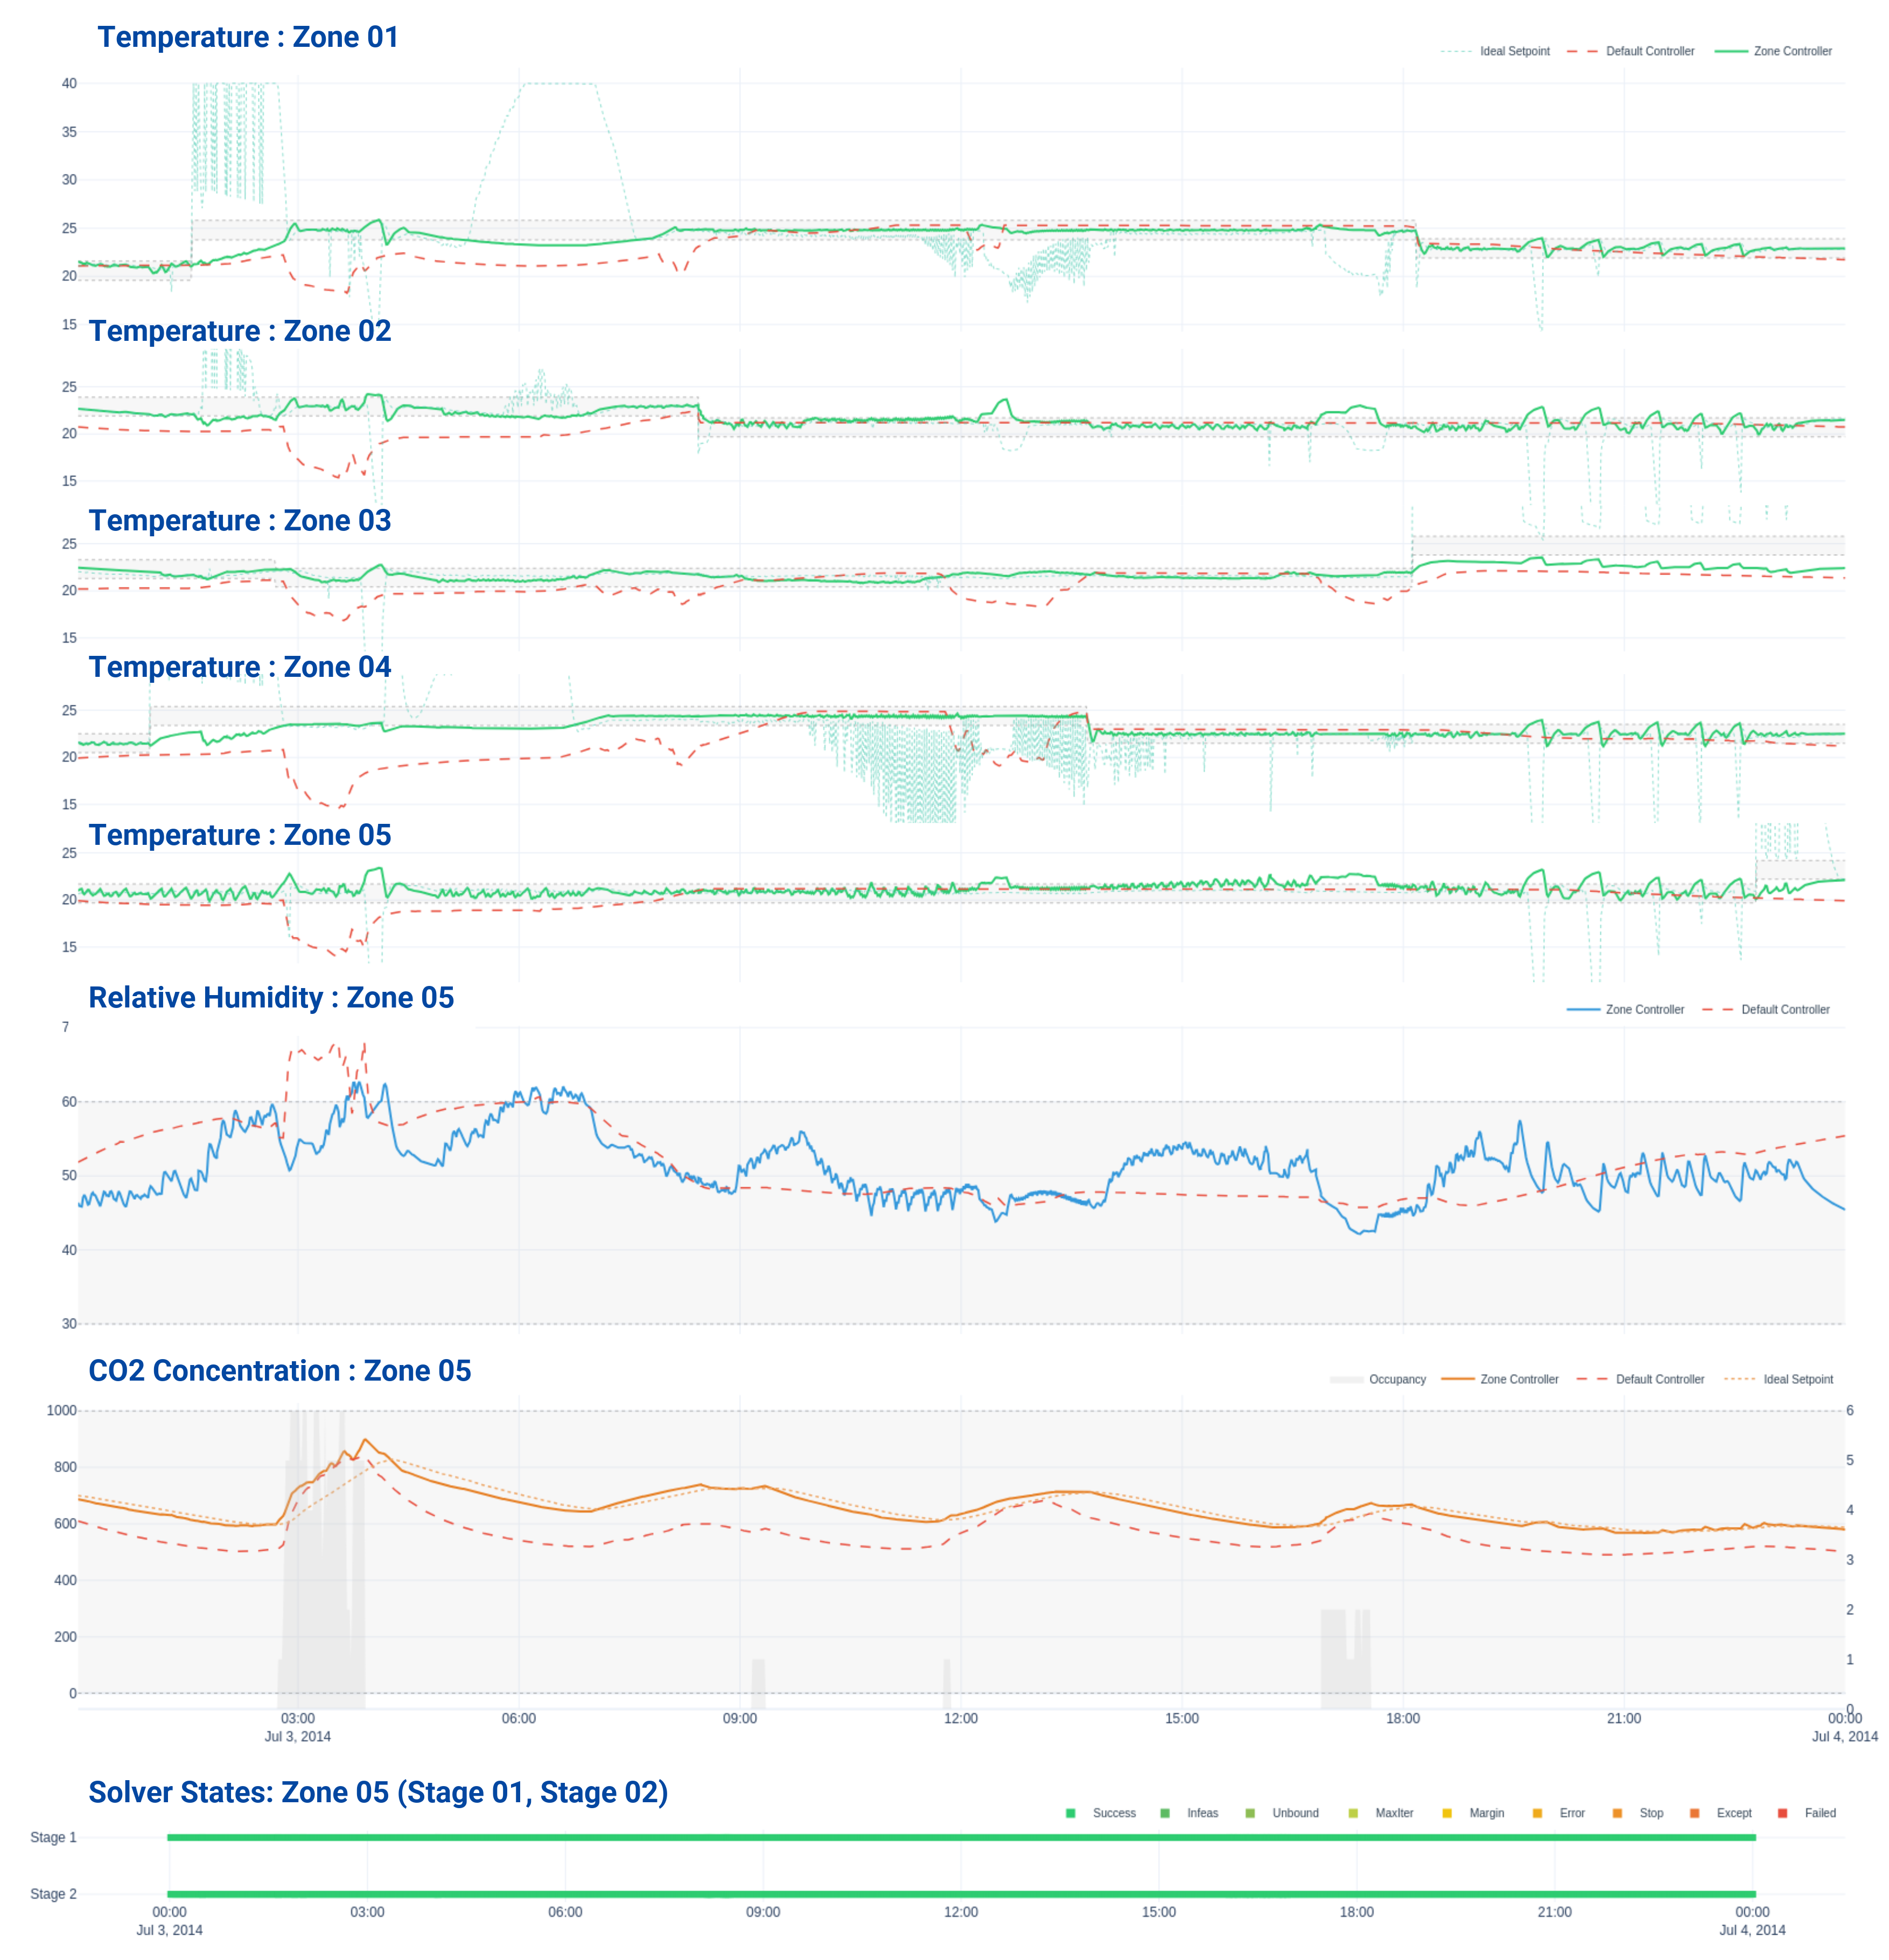
\includegraphics[width=\linewidth]{results/fig_sim_allzone_temp.png}
		\caption{Temperature regulation across all five zones over the full
			31-day simulation}
		\label{fig:allzone_temp}
	\end{figure}
	
	Table~\ref{tab:zone_perf} compares the proposed decentralised Zone Controller with the EnergyPlus default controller over the 31-day simulation period during scheduled occupancy hours. The comparison should be interpreted in the context of the information and actuation available to each controller. The EnergyPlus default controller represents a highly informed reference implementation. It operates with the exact system parameters available within the simulation environment and has direct access to the simulated system states and model information. In addition, its centralised HVAC control structure can coordinate the plant and exploit zone-level reheat, providing an inherent advantage in maintaining humidity and temperature conditions.
	
	In contrast, the proposed controller operates using only the measurements available from the zone sensors, with the controller receiving sensor equivalent values extracted from the simulation environment rather than direct access to the underlying EnergyPlus system states or exact plant parameters. The proposed architecture must therefore estimate unmeasured states and disturbances online through the EKF and coordinate the zones through its decentralised control structure.
	
	Despite these differences, the proposed controller achieves substantially improved temperature regulation across the five zones, with temperature in-range performance increasing from 62.5\%, 37.2\%, 24.9\%, 38.1\%, and 41.9\% under the default controller to 68.9\%, 84.9\%, 85.4\%, 74.7\%, and 87.0\%, respectively. The lower humidity in range percentages under the proposed controller should not be interpreted independently of the control objectives, the default system benefits from its centralised knowledge and zone level reheat capability, which provides additional authority for humidity management. Still, the proposed controller maintains the prescribed humidity region while simultaneously regulating temperature and CO$_2$ using its available airflow-based actuation.

	CO$_2$ regulation is also maintained at the required level for 99.2--100\% of occupied time across all zones. Overall, the results demonstrate that the proposed decentralised architecture can achieve comparable multi-variable comfort and IAQ performance to a highly informed centralised system, despite operating with sensor level information and without the same degree of model knowledge and actuator coordination. This provides evidence that the decentralised formulation can retain much of the control performance of a centralised approach while offering a more scalable control structure for increasing numbers of zones.
	
	\begin{table}[htbp]
		\centering
		\small
		\caption{Zone controller performance summary - proposed (P) vs.
			default EnergyPlus controller (D)}
		\label{tab:zone_perf}
		\begin{tabular}{lrrrrrrrrrrr}
			\toprule
			\textbf{Metric}
			& \multicolumn{2}{c}{\textbf{SP1-1}}
			& \multicolumn{2}{c}{\textbf{SP2-1}}
			& \multicolumn{2}{c}{\textbf{SP3-1}}
			& \multicolumn{2}{c}{\textbf{SP4-1}}
			& \multicolumn{2}{c}{\textbf{SP5-1}} \\
			\cmidrule(lr){2-3}\cmidrule(lr){4-5}\cmidrule(lr){6-7}
			\cmidrule(lr){8-9}\cmidrule(lr){10-11}
			& P & D & P & D & P & D & P & D & P & D \\
			\midrule
			MAE $T$ ($^\circ$C)     & 1.12 & 1.35 & 1.12 & 1.70 & 1.26 & 1.44 & 1.33 & 1.13 & 1.27 & 2.17 \\
			\% $T$ in range         & 68.9 & 62.5 & 84.9 & 37.2 & 85.4 & 24.9 & 74.7 & 38.1 & 87.0 & 41.9 \\
			\% RH in range          & 89.9 & 100  & 87.7 & 100  & 89.9 & 100  & 89.2 & 100  & 88.0 & 100  \\
			Max CO$_2$ (ppm)        &  967 &  849 &  912 &  836 &  984 &  840 &  910 &  850 & 1037 &  840 \\
			\% CO$_2$ in range      & 100  & 100  & 100  & 100  & 100  & 100  & 100  & 100  & 99.2 & 100  \\
			\bottomrule
		\end{tabular}
	\end{table}
	
	\subsubsection{AHU Coordinator Arbitration}
	
	Figure~\ref{fig:ahu_arbitration} shows the AHU Coordinator arbitration
	signals for a representative 24-hour window, during which
	zone occupancy transitions from the night setback period through the
	morning peak and into the afternoon.
	
	Several behaviours confirm correct coordinator operation.  The
	commanded temperature setpoint remains inside the arbitration envelope
	at all times, demonstrating that the weighted-least-squares arbitration
	never overrides the extreme zone requests but instead finds a feasible
	central operating point.  The CO$_2$ setpoint tracks the zone demand
	aggregate closely during occupied hours, rising from the outdoor-air
	baseline near 600~ppm during unoccupied periods to approximately
	750-850~ppm as zones fill.  The economizer mix ratio $\gamma$ stays
	near zero for most of the time and add minimal outdoor air when the supply
	is already close to the neutral condition and rises during	hours when outdoor conditions are cooler, confirming that the energy	penalty term in the coordinator objective is correctly discouraging
	unnecessary mechanical cooling.  The optimizer status strip at
	the bottom shows all timesteps solved as QP successes, confirming
	computational tractability throughout.
	
	\begin{figure}[htbp]
		\centering
		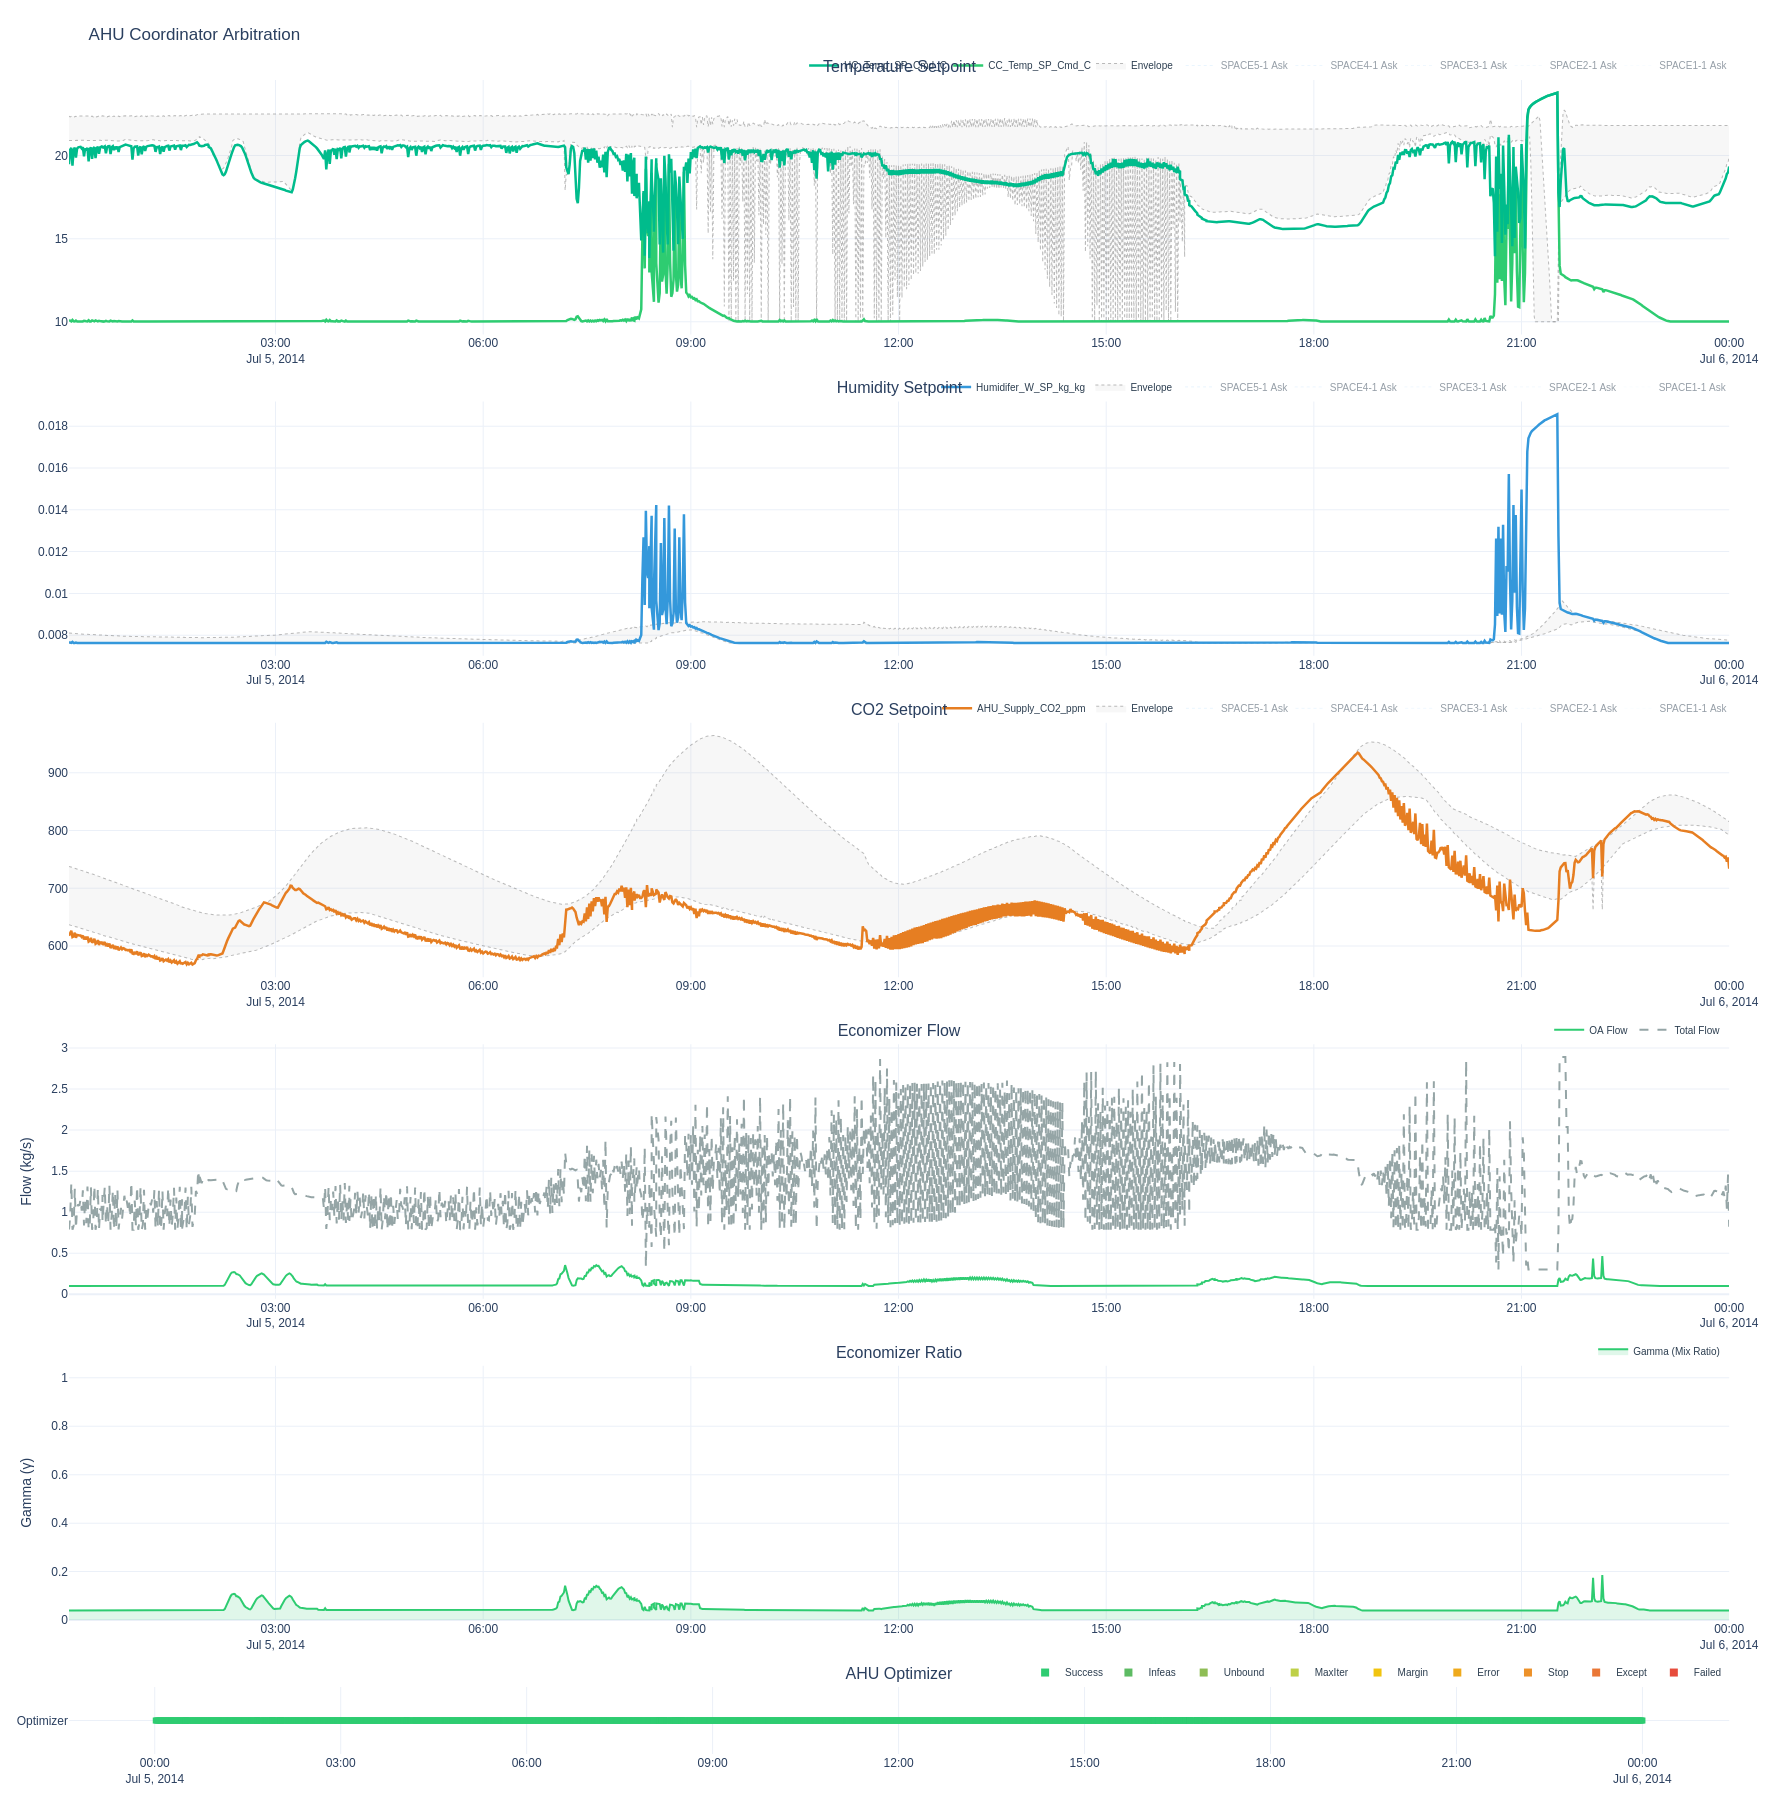
\includegraphics[width=\linewidth]{results/fig_sim_ahu_arbitration.png}
		\caption{AHU Coordinator arbitration for a representative 24-hour
			period }
		\label{fig:ahu_arbitration}
	\end{figure}
	
	\newpage
	\subsubsection{Overall Simulation Results}
	
	Figure~\ref{fig:comfort_bars} presents the overall simulation results for the proposed decentralised Zone Controller across all five zones. The results are evaluated against the comfort and IAQ operating regions defined for temperature, relative humidity, and CO$_2$. The combined results illustrate the controller's ability to maintain the three coupled IAQ variables within their respective limits under varying zone conditions and disturbances.
	
		\begin{figure}[htbp]
		\centering
		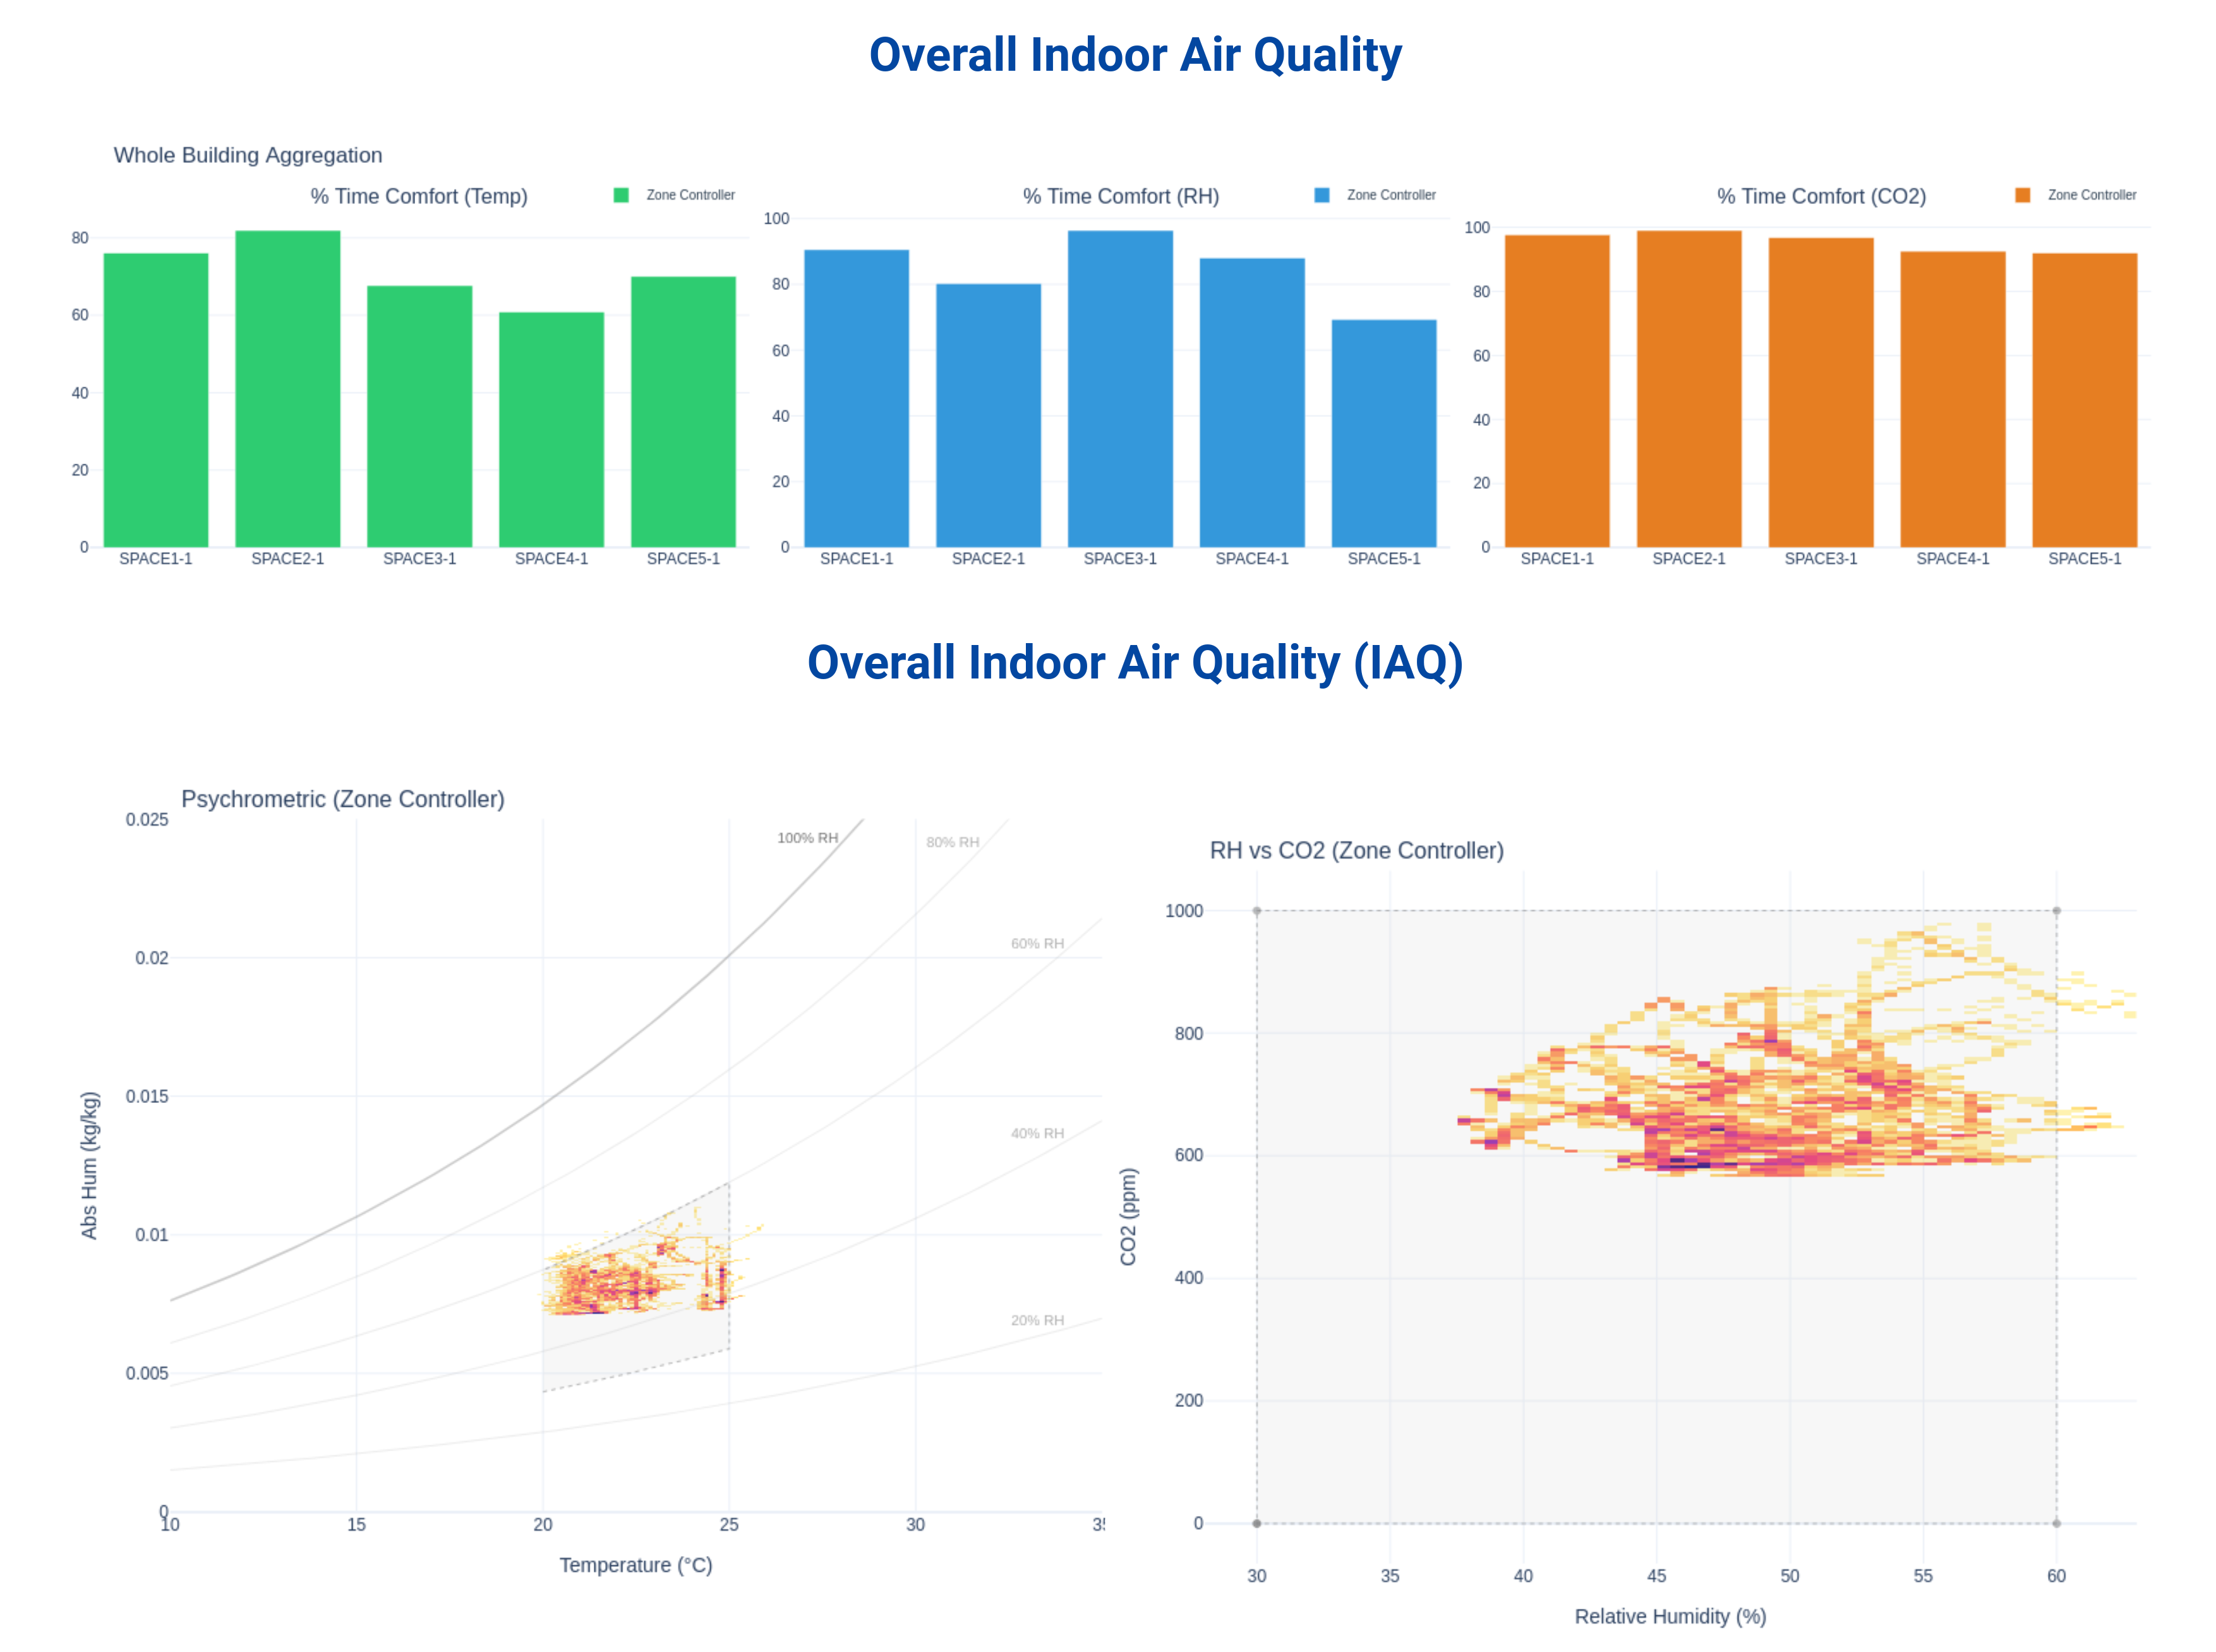
\includegraphics[width=\linewidth]{results/fig_sim_comfort_bars.png}
		\caption{Whole-building comfort aggregation}
		\label{fig:comfort_bars}
	\end{figure}
	
	The psychrometric plot shows that the majority of the operating points from all five zones remain within the defined temperature--humidity comfort region. This demonstrates that the controller is able to simultaneously regulate sensible and latent conditions using the available airflow actuator, despite the different dynamics of temperature and humidity. The RH--CO$_2$ plot further shows that the operating conditions remain within the specified IAQ region, with relative humidity maintained between the prescribed 30-60\%~RH limits and CO$_2$ concentrations generally remaining below the 1000~ppm ceiling.
		

	
	\newpage
	% ------------------------------------------------------------
	\subsection{Single-Zone Cool Room Experimental Performance and Hardware
		Validation}
	\label{sec:results_exp}
	% ------------------------------------------------------------
	
	The EnergyPlus simulation validates the architecture against a
	high fidelity building model, but confirmation that the same control
	algorithms execute correctly on embedded hardware under real sensor
	noise, communication latency, and unmodelled AHU dynamics is essential
	to close the deployment gap identified in Chapter~2.
	The following results were recorded on the physical single-zone cool
	room testbench described in Section 4, running the DECEN-VAV
	firmware.
	

	
	\subsubsection{Zone Controller Performance}
	
	Figure~\ref{fig:exp_zone} shows the zone-level performance of the
	Zone Controller on the physical testbench.
	
	The room temperature converges from an initial value of approximately
	24.5$^\circ$C to within 1$^\circ$C of the 22$^\circ$C setpoint
	within 20~minutes of controller activation, and remains within the
	$\pm 1^\circ$C deadband for the remainder of the session.  The
	relative humidity decreases steadily from 80\%~RH at startup to
	approximately 50--55\%~RH during steady-state operation, remaining
	within the 30--60\%~RH comfort band after the initial transient.
	The CO$_2$ concentration in the adjacent rooms stays below 600~ppm
	throughout, well within the 1000~ppm IAQ ceiling, confirming adequate
	outdoor-air ventilation.
	
	The psychrometric scatter plot in the lower-left panel shows the
	zone operating trajectory converging from the warm, humid upper-right
	region of the chart toward the shaded comfort rectangle, where it
	remains tightly clustered during steady-state.  The RH--CO$_2$
	joint density confirms simultaneous satisfaction of the humidity
	and CO$_2$ constraints: the operating cloud is centred inside the
	comfort rectangle (30--60\% RH, $<$~1000~ppm), with no sustained
	excursions beyond its boundaries.
	
	These experimental results confirm that the EKF, zone MPC, supply-state
	solver, and flow-authority taper all execute correctly on the ESP32
	embedded hardware, and that the control algorithms transfer from the
	EnergyPlus simulation environment to a physical AHU without loss of
	stability or comfort performance.
	
	\begin{figure}[htbp]
	\centering
	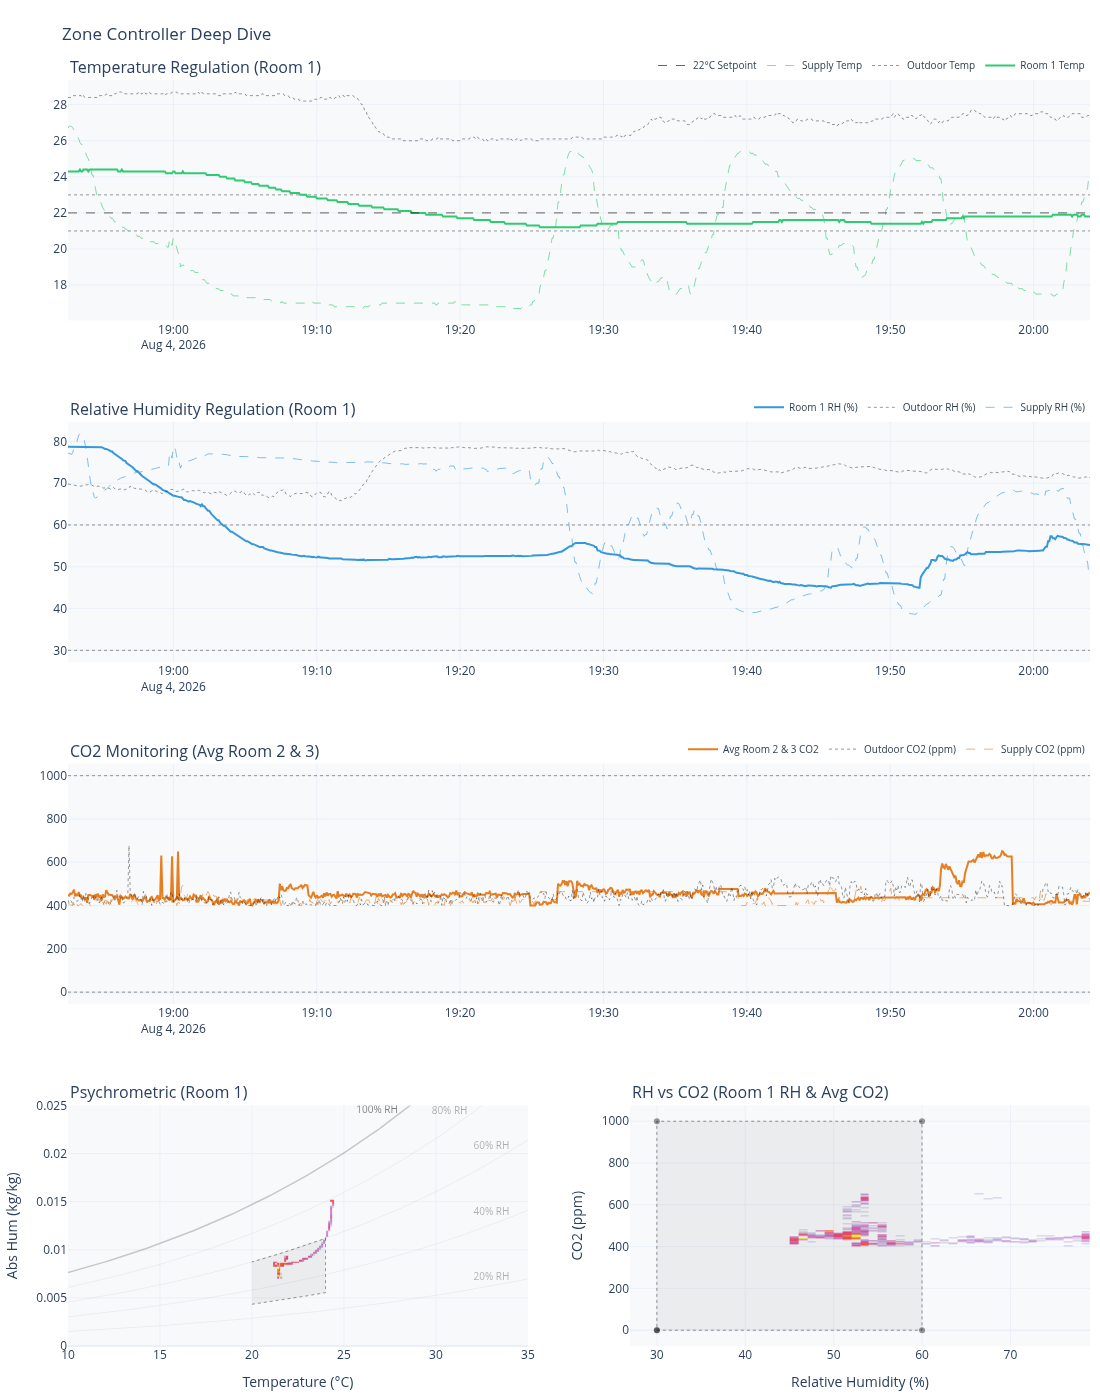
\includegraphics[width=\linewidth]{results/fig_exp_zone_deepdive.png}
	\caption{Zone Controller on the physical testbench.}
	\label{fig:exp_zone}
	\end{figure}
	
	\subsubsection{AHU Coordinator Arbitration on Hardware}
	
	Figure~\ref{fig:exp_ahu_arb} shows the AHU-level arbitration
	signals recorded during the session.
	
	\begin{figure}[htbp]
		\centering
		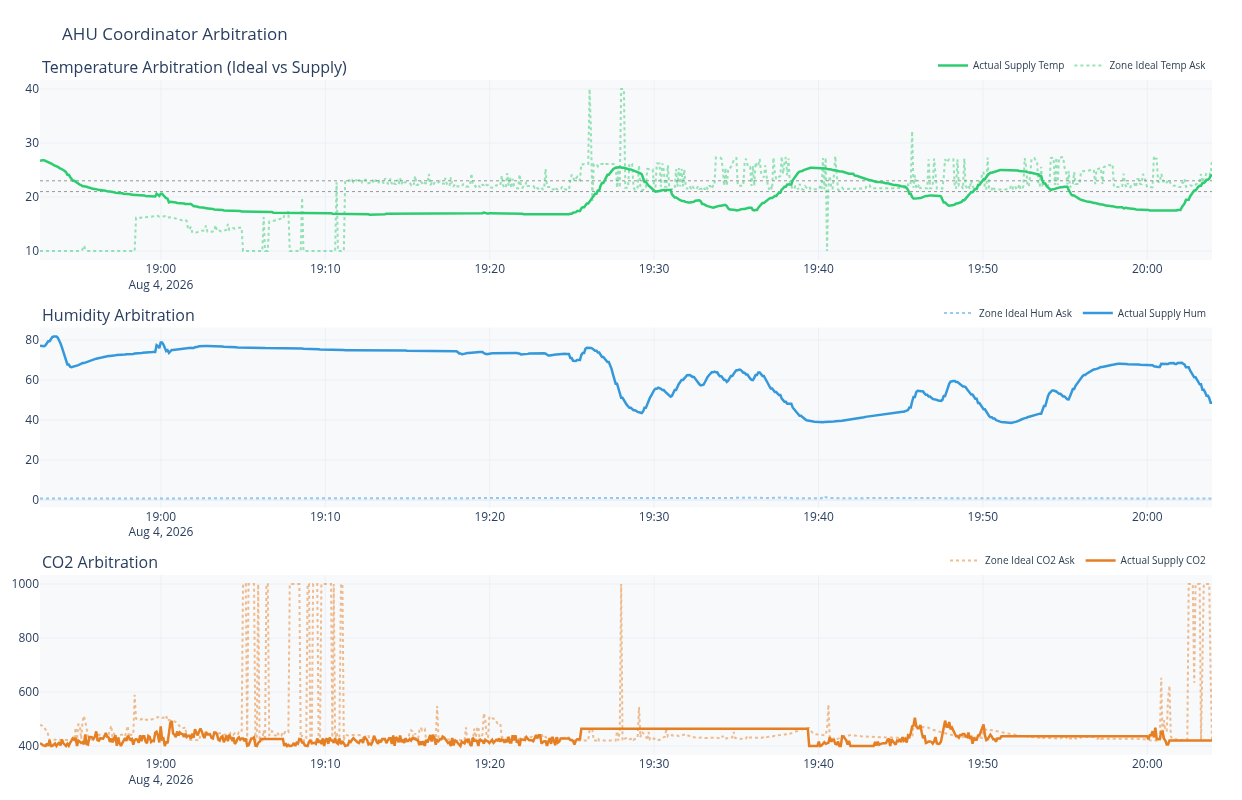
\includegraphics[width=\linewidth]{results/fig_exp_ahu_arb.png}
		\caption{Hardware AHU coordinator arbitration}
		\label{fig:exp_ahu_arb}
	\end{figure}
	
	The supply temperature tracks the zone requests throughout the window.  The early portion of the trace
	(18:55--19:15) shows the cool room initialising from a warm state,
	the zone controller immediately requests a sub neutral supply
	temperature, and the coordinator responds by turning on the cooling
	coil.  After the zone stabilises near 22$^\circ$C the coordinator
	relaxes the cooling setpoint toward the neutral mixed-air condition,
	consistent with the energy penalty term in the coordinator
	objective.  The CO$_2$
	arbitration confirms that the outdoor air fraction is held at the
	minimum ventilation level during unoccupied hours, with supply
	CO$_2$ near the outdoor ambient concentration of approximately
	420~ppm.
	
	\subsubsection{AHU Component Actuation}
	
	Figure~\ref{fig:exp_actuation} shows the raw actuator command signals
	sent by the embedded controller to the AHU hardware components
	during the same window.
	
	\begin{figure}[htbp]
		\centering
		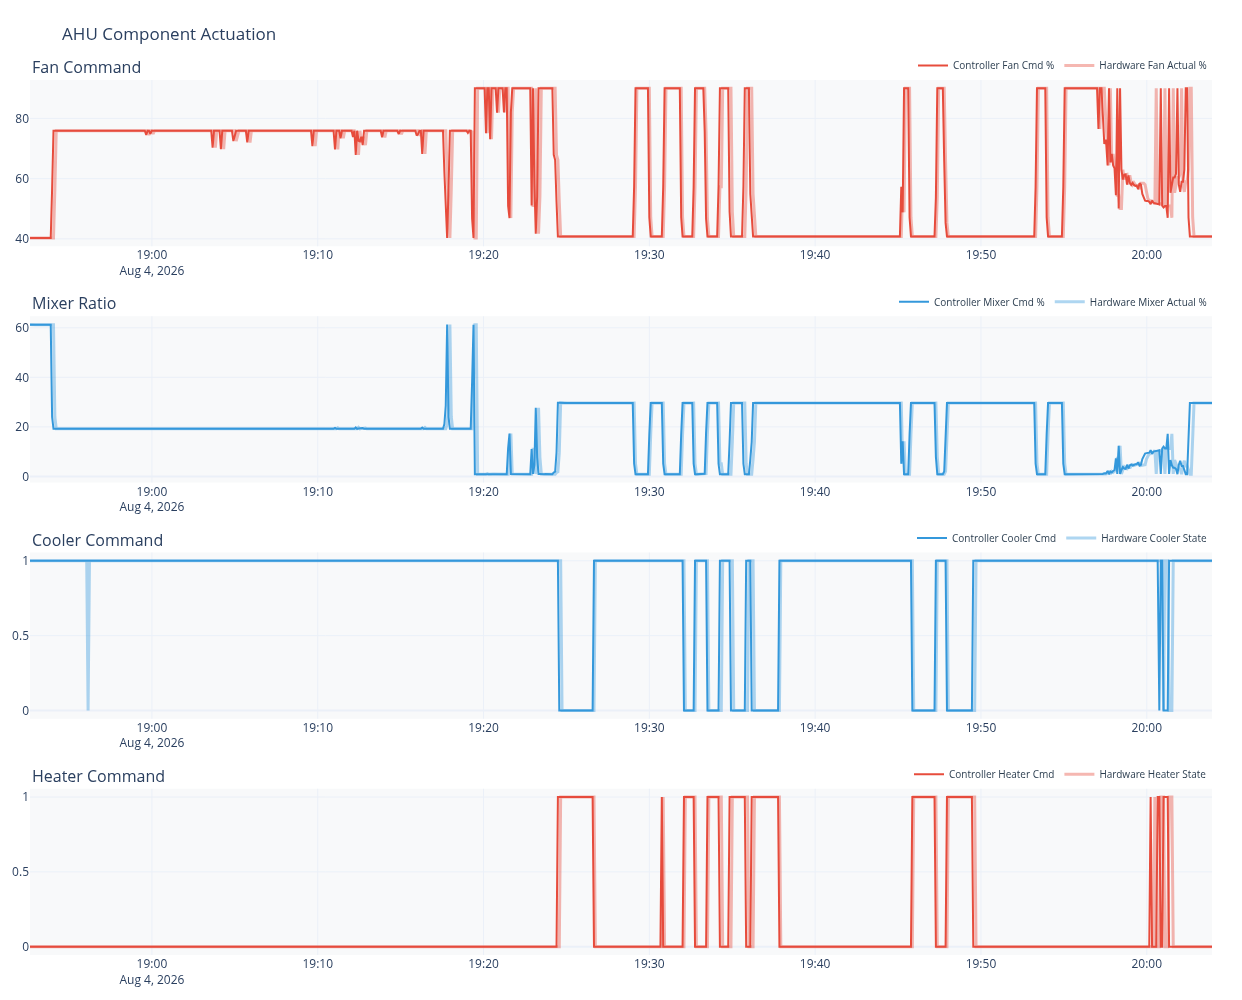
\includegraphics[width=\linewidth]{results/fig_exp_actuation.png}
		\caption{AHU component actuation on the physical testbench}
		\label{fig:exp_actuation}
	\end{figure}
	
	The fan command operates between 40\% and 90\% PWM, tracking
	the VAV flow demand computed by the zone MPC.  The mixer ratio
	varies between 0\% and 60\% in response to the coordinator's
	outdoor-air fraction command, with brief transients during setpoint
	changes.  The cooler relay engages during the initial cooling
	phase and then cycles at a lower duty cycle once the zone stabilises,
	consistent with the flow-authority taper reducing the aggressiveness
	of the supply request as the zone approaches comfort bounds.  The
	heater relay activates briefly during the 19:20-19:35 period when
	the coordinator determines that a warm supply is required to counteract
	a drop below the temperature deadband floor.  The hardware relay
	states follow the controller commands with a latency of one to two
	control timesteps, which falls within 	the prediction horizon of the zone MPC and does not cause instability.


\newpage
\section{Discussion}

\subsection{Modelling Challenges and Grey-Box Model Development}

A major challenge was developing a control-oriented model that retained physical meaning while remaining identifiable from available sensor data. A fully white-box model would require detailed building information that is generally unavailable, while a black-box model would require extensive training data and provide limited physical interpretability. The selected 2R2C grey-box model provides a practical compromise, with its thermal resistances and capacitances estimated online through the augmented EKF.

Parameter identifiability was initially challenging because different parameter combinations can produce similar temperature responses during periods of low disturbance. This was addressed by modelling the parameters as slowly varying EKF states with appropriately tuned process noise. The EKF covariance diagnostics showed rapid convergence followed by stable estimates, indicating successful joint estimation of building parameters and disturbances.

\subsection{EKF Tuning and Convergence}

EKF tuning required balancing the different dynamics of physical states, disturbances, and parameters. Disturbance states were assigned sufficient process noise to track changes in occupancy, solar gains, and other unmeasured inputs, while parameter states used much smaller values to prevent unrealistic drift. Multiple validation cycles were required before consistent convergence was obtained across all five zones.

\subsection{MPC Tuning and Constraint Hierarchy}

The two phase MPC required careful tuning of actuation, comfort, and constraint-violation weights. Comfort constraints were given priority over airflow minimisation, while deadband centering terms were introduced to prevent switching between minimum and maximum airflow near constraint boundaries. Humidity regulation required particular attention because its response to airflow is slower and more nonlinear than temperature. The sequential linearisation strategy separates flow optimisation from supply-state optimisation, avoiding the non-convexity of their bilinear coupling. Although this introduces some sub-optimality, it remained effective  within the operating range considered.

\subsection{PCB Design and Sensor Noise Mitigation}

The initial breadboard implementation introduced electrical noise on the I2C bus, causing fluctuations in the BME280 and ENS160 measurements that affected EKF estimation. A custom PCB was therefore developed with improved trace routing, common grounding, and power decoupling. This substantially reduced measurement noise while also improving the reliability of the hardware.

\subsection{Sensor Placement and Multi-Sensor Averaging}

Sensor placement was found to significantly affect the measured zone conditions because temperature, humidity, and CO$_2$ are not spatially uniform. Sensors positioned near supply or return air streams produced biased measurements relative to the well-mixed zone assumption. Mid-height placement near the zone centroid provided more representative measurements. Therefore, multiple sensor nodes were averaged before the EKF update. This reduced the influence of local variations and effectively lowered measurement noise without requiring a more complex filters.

\subsection{Simulation-to-Hardware Transfer}

The control algorithms transferred from EnergyPlus to the physical testbench without controller retuning. The physical system achieved temperature convergence to within $1\,^\circ$C of the setpoint within 20 minutes and maintained the prescribed IAQ variables during steady-state operation. Hardware actuation delays of one to two control timesteps remained within the MPC prediction horizon and did not cause instability. The calibrated fan-flow model also provided sufficient accuracy for converting the MPC airflow command into fan-speed commands.


\newpage
\section{Conclusions}

This project developed, implemented, and validated a decentralised control architecture for multi-zone HVAC systems that jointly regulates indoor temperature, relative humidity, and CO$_2$ within prescribed comfort and IAQ limits. The work addresses three key challenges, 
\begin{enumerate}
	\item Computational growth of centralised MPC with increasing zone count.
	\item Underactuated joint control of temperature, humidity, and CO$_2$ through a single VAV actuator.
	\item Gap between simulation-based control designs and practical hardware deployment.
\end{enumerate}

Five-zone EnergyPlus validation showed improved temperature in range performance across all zones, increasing from 24.9-62.5\% under the default controller to 68.9-87.0\% with the proposed controller. CO$_2$ remained below the 1000~ppm limit for 99.2--100\% of occupied hours. These results are particularly significant because the proposed controller operates using sensor equivalent measurements rather than direct access to the underlying simulation states or zone-level reheat available to the default controller. Physical validation on the single-zone testbench further demonstrated successful execution on ESP32 hardware under sensor noise, communication delays, and unmodelled plant dynamics. Temperature converged within the $\pm1\,^\circ$C deadband within 20 minutes, while humidity and CO$_2$ remained within their prescribed limits during steady-state operation.

Overall, the work demonstrates a practical decentralised framework for multivariable IAQ control in which zone-level estimation and optimisation are distributed while shared AHU resources remain centrally coordinated. Its modular structure allows additional zones to be incorporated without redesigning the existing zone controllers, providing a practical basis for extending advanced IAQ control to larger multi-zone HVAC systems.

\newpage
\section{Future Work}

\subsection{Multi-Zone Hardware Deployment and Robustness Testing}

The next step is to deploy the complete two-layer architecture on a physical multi-zone testbench. While the five-zone EnergyPlus results demonstrate the decentralised structure, physical validation was limited to a single zone. A multi-zone implementation would allow evaluation of real inter-zone coupling, network communication, and AHU arbitration under competing zone requests. Further testing should also examine sensor failures, communication dropouts, and abrupt occupancy changes to assess robustness and graceful degradation.

\subsection{System Tuning}

The current implementation requires manual tuning of initial EKF covariance and process-noise parameters. Future work should develop an automated commissioning procedure using structured excitation or historical sensor data to identify suitable grey-box parameters before controller activation. This would reduce building-specific setup and move the framework toward more automated deployment across different buildings and climates.

\subsection{VAV Systems with Reheat Terminals}

The present work considers a no-reheat VAV configuration, requiring temperature, humidity, and CO$_2$ regulation through the VAV airflow actuator. Extending the Zone Controller to include terminal reheat as an additional decision variable would provide greater control authority where such hardware is available. The resulting formulation could retain the existing no-reheat strategy while exploiting reheat when required for improved multivariable regulation.

\subsection{Demand Response and Energy Aware Control}

The supervisory formulation provides a basis for future energy aware extensions such as time varying electricity prices or demand response signals could be incorporated into the AHU Coordinator objective, allowing thermal loads to be shifted while maintaining the prescribed comfort and IAQ constraints.
	
	\newpage
	
	% ==========================================
	% BACK MATTER
	% ==========================================
	
	\bibliographystyle{apalike}
	\bibliography{ref}

	\newpage
	
	% --- APPENDICES ---
	\appendix
	\section{Nomenclature \& Variable Definitions}
	
	\subsection*{State \& Output Variables}
	\begin{description}[align=left, labelwidth=2.5cm, leftmargin=!]
		\item[$x$] State vector of the zone
		\item[$y$] Output measurement vector of the zone
		\item[$T_{\mathrm{in}}$] Indoor air temperature [$^\circ\mathrm{C}$]
		\item[$T_m$] Temperature of the building's thermal mass [$^\circ\mathrm{C}$]
		\item[$W_{\mathrm{in}}$] Indoor humidity ratio [$\mathrm{kg_w/kg_{da}}$]
		\item[$C_{\mathrm{in}}$] Indoor $\mathrm{CO}_2$ concentration [$\mathrm{mg/m^3}$]
	\end{description}
	
	\subsection*{Control \& Supply Parameters (AHU)}
	\begin{description}[align=left, labelwidth=2.5cm, leftmargin=!]
		\item[$u$] Control input representing VAV volumetric flow rate $\dot{V}_s$ [$\mathrm{m^3/s}$]
		\item[$\dot{V}_s$] Volumetric flow rate of supply air [$\mathrm{m^3/s}$]
		\item[$T_s$] Supply air temperature [$^\circ\mathrm{C}$]
		\item[$W_s$] Supply air humidity ratio [$\mathrm{kg_w/kg_{da}}$]
		\item[$C_s$] Supply air $\mathrm{CO}_2$ concentration [$\mathrm{mg/m^3}$]
	\end{description}
	
	\subsection*{Physical Constants \& Geometric Parameters}
	\begin{description}[align=left, labelwidth=2.5cm, leftmargin=!]
		\item[$C_{\mathrm{air}}$] Thermal capacitance of the room's air volume [$\mathrm{J/K}$]
		\item[$C_{\mathrm{mass}}$] Thermal capacitance of the building's solid mass [$\mathrm{J/K}$]
		\item[$M_{\mathrm{air}}$] Total mass of dry air inside the room [$\mathrm{kg_{da}}$]
		\item[$V_{\mathrm{room}}$] Total volume of the room [$\mathrm{m^3}$]
		\item[$R_{\mathrm{ext}}$] Thermal resistance of the external building envelope [$\mathrm{K/W}$]
		\item[$R_{\mathrm{int}}$] Internal thermal resistance between the indoor air and building mass [$\mathrm{K/W}$]
		\item[$\rho_{\mathrm{air}}$] Density of the air [$\mathrm{kg/m^3}$]
		\item[$c_p$] Specific heat capacity of the air [$\mathrm{J/(kg \cdot K)}$]
	\end{description}
	
	\subsection*{Disturbances \& Heuristic Estimations}
	\begin{description}[align=left, labelwidth=2.5cm, leftmargin=!]
		\item[$N_{\mathrm{occ}}$] Estimated number of occupants
		\item[$Q_{\mathrm{equip}}$] Estimated equipment sensible heat gain [$\mathrm{W}$]
		\item[$q_{\mathrm{person}}$] Standard sensible heat generation per occupant [$\mathrm{W/person}$]
		\item[$g_{w,\mathrm{person}}$] Standard moisture generation per occupant [$\mathrm{kg_w/(s \cdot person)}$]
		\item[$g_{\mathrm{co2,person}}$] Standard $\mathrm{CO}_2$ generation per occupant [$\mathrm{mg/(s \cdot person)}$]
		\item[$d_T$] Lumped thermal disturbance [$\mathrm{W}$]
		\item[$d_W$] Lumped moisture disturbance [$\mathrm{kg_w/s}$]
		\item[$d_C$] Lumped $\mathrm{CO}_2$ disturbance [$\mathrm{mg/s}$]
	\end{description}
	
	
	
\end{document}